\title{CS313 : DataBases and Information Systems Lab\\
    \vspace{0.6cm}
    Assignment 6 (Project 1) 
} % You may change the title if you want.
% \subtitle{Hello}
\author{Sourabh Bhosale \\ 200010004}

\date{\today}

\documentclass[12pt]{article}
\usepackage{fullpage}
\usepackage{enumitem}
\usepackage{amsmath,mathtools}
\usepackage{amssymb}
\usepackage[super]{nth}
\usepackage{textcomp}
\usepackage{hyperref}
\usepackage{multicol}
\usepackage{multirow}
\usepackage{minted}
\usepackage{xcolor}
% \renewcommand{\baselinestretch}{1.22}
% \tolerance=1
% \emergencystretch=\maxdimen
% \hyphenpenalty=10000
% \hbadness=10000
% \definecolor{code_gray}{rgb}{0.8,0.8,0.8}
\definecolor{bgcolor}{HTML}{E0E0E0}
\let\oldtexttt\texttt
\renewcommand{\texttt}[1]{
  \colorbox{bgcolor}{\oldtexttt{#1}}
  }

% \usepackage{fontspec}
% \usepackage[showframe]{geometry}

% \usepackage[default,oldstyle,scale=0.95]{helvet}
% \usepackage[T1]{fontenc}

% \usepackage{merriweather}
% \usepackage[T1]{fontenc}

% \usepackage[sfdefault]{noto}
% \usepackage[T1]{fontenc}

\usepackage[default,oldstyle,scale=0.95]{opensans} %% Alternatively
%% use the option 'defaultsans' instead of 'default' to replace the
%% sans serif font only.
\usepackage[T1]{fontenc}

% \usepackage[scaled]{helvet} 
% \setmainfont{Roboto}
\usepackage{titling}
\hypersetup{
    colorlinks=true,
    linkcolor=blue,
    filecolor=magenta,      
    urlcolor=cyan,
}

\renewcommand\maketitlehooka{\null\mbox{}\vfill}
\renewcommand\maketitlehookd{\vfill\null}

\begin{document}


\begin{titlingpage}
\maketitle
\end{titlingpage}

\newpage
%---------------------------------------------------------------------

% \begin{tiny}
\section{Part A: J2EE Project}

All the program related to part A is inside the \texttt{Part\_A/J2EEProject} directory.

\subsection{Executing the sample project given (J2EEProject.zip) and understanding the execution flow.}

\begin{figure}[!hbt]
    \centering
    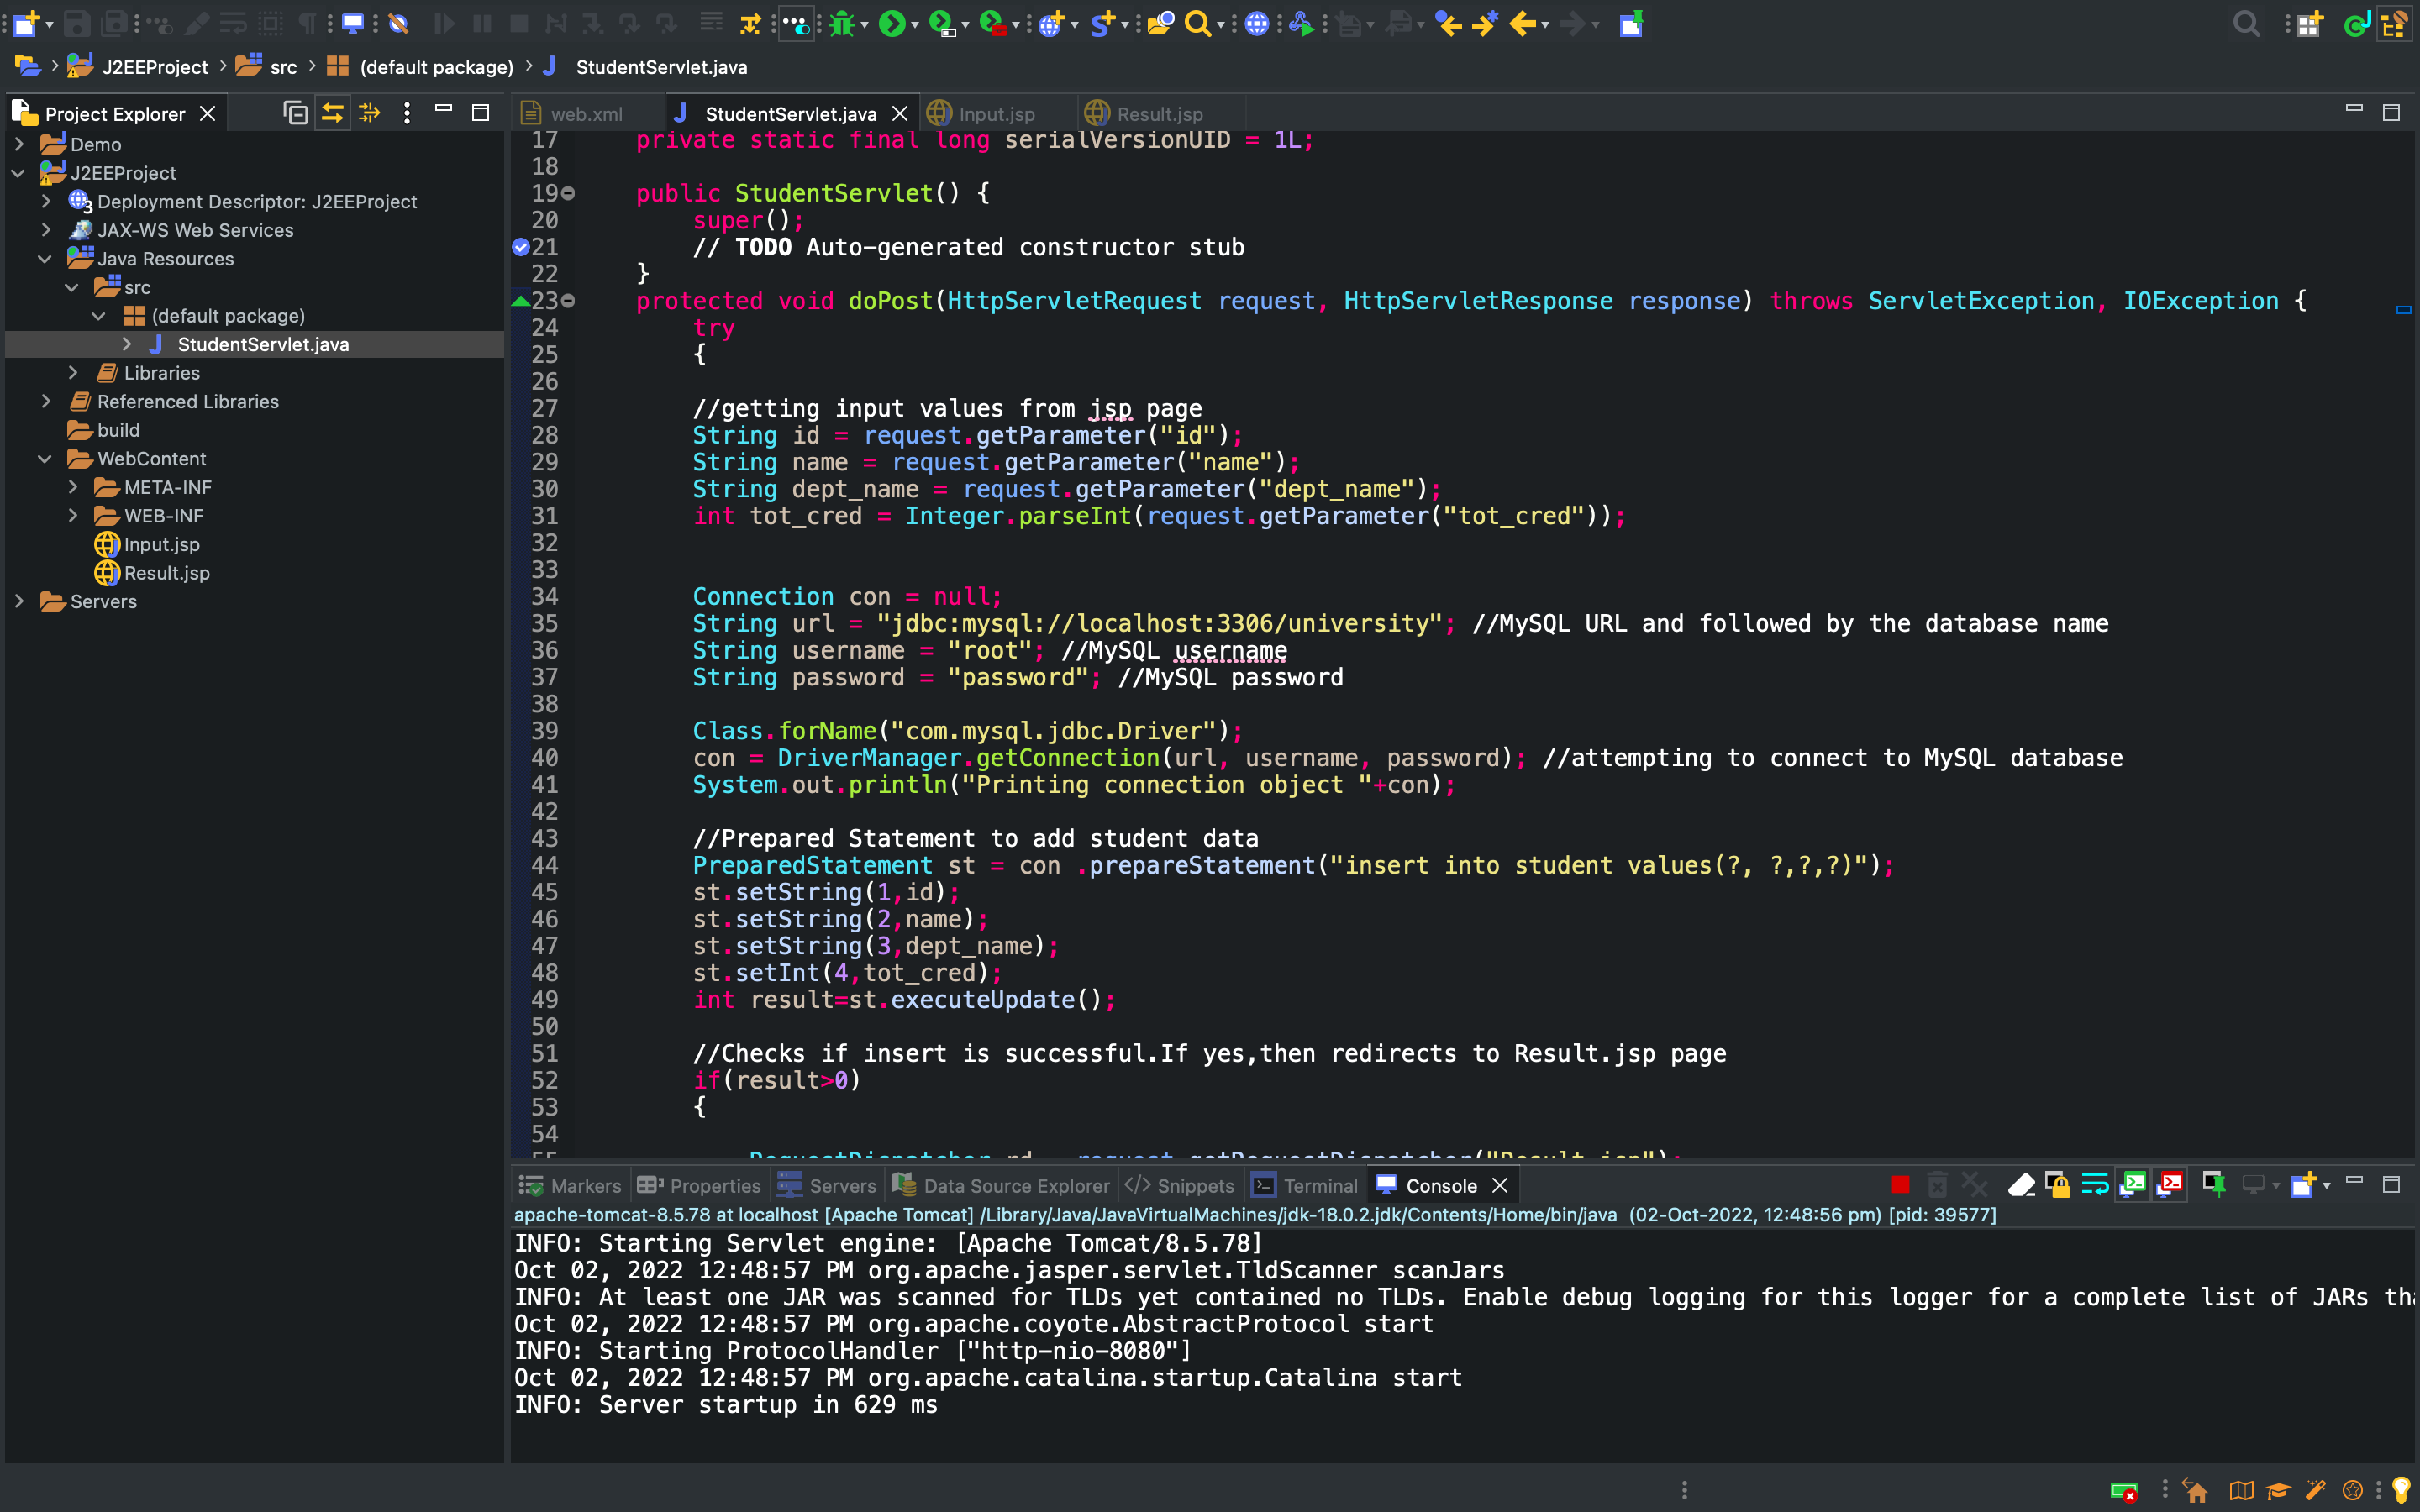
\includegraphics[scale=0.3]{screenshots/a11.png}
    \label{fig:my_label1}
    \caption{IDE Screenshot}
\end{figure}

\begin{figure}[!hbt]
    \centering
    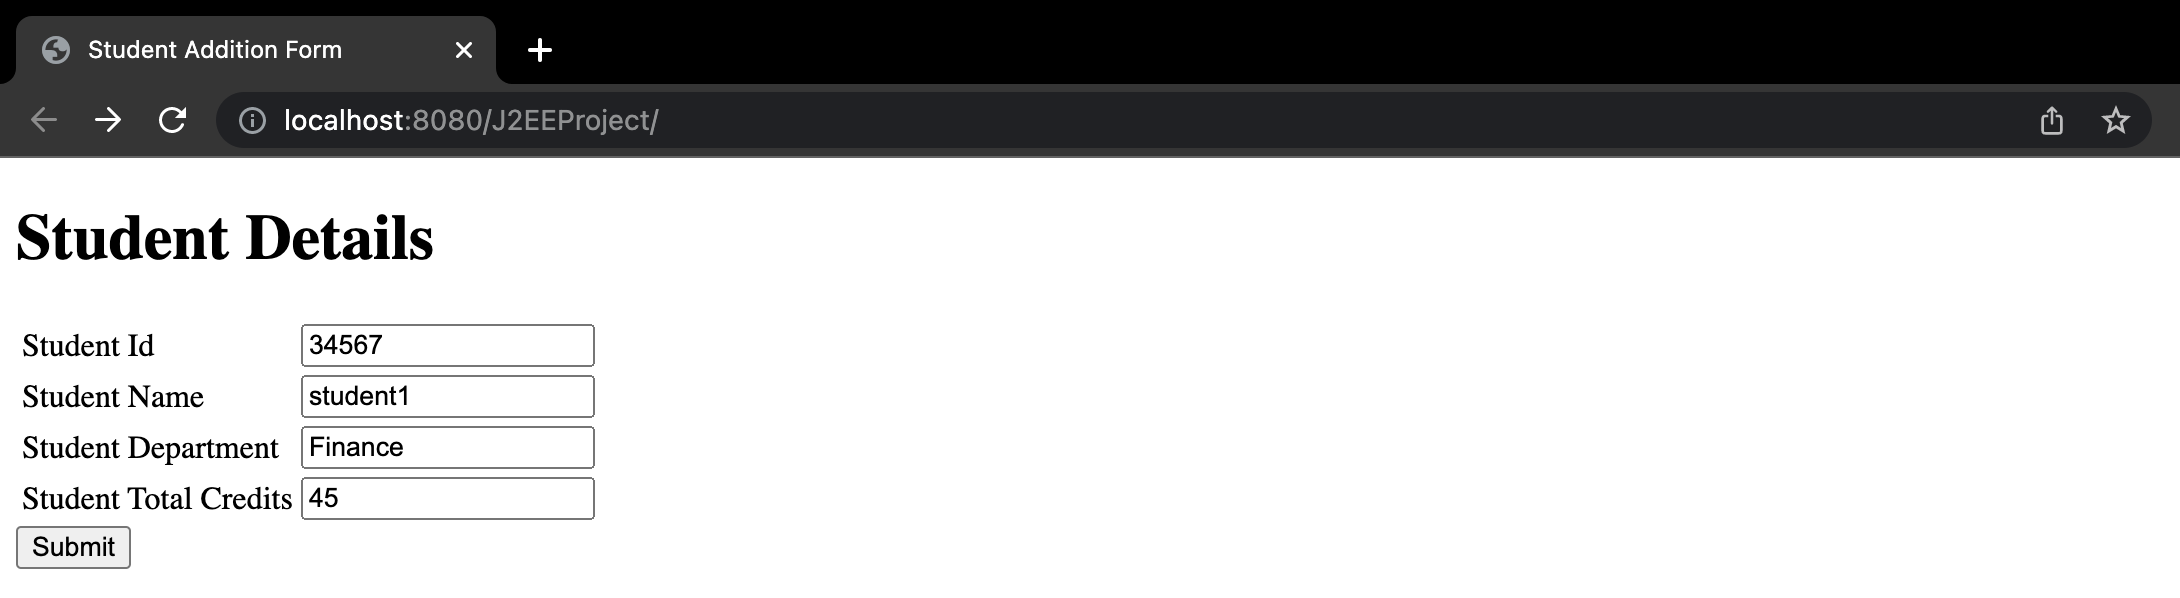
\includegraphics[scale=0.42]{screenshots/a12.png}
    \label{fig:my_label1}
    \caption{Data Insertion}
\end{figure}

\newpage

\begin{figure}[!hbt]
    \centering
    
\includegraphics[scale=0.4]{screenshots/a13.png}
    \label{fig:my_label1}
    \caption{Result}
\end{figure}

\begin{figure}[!hbt]
    \centering
    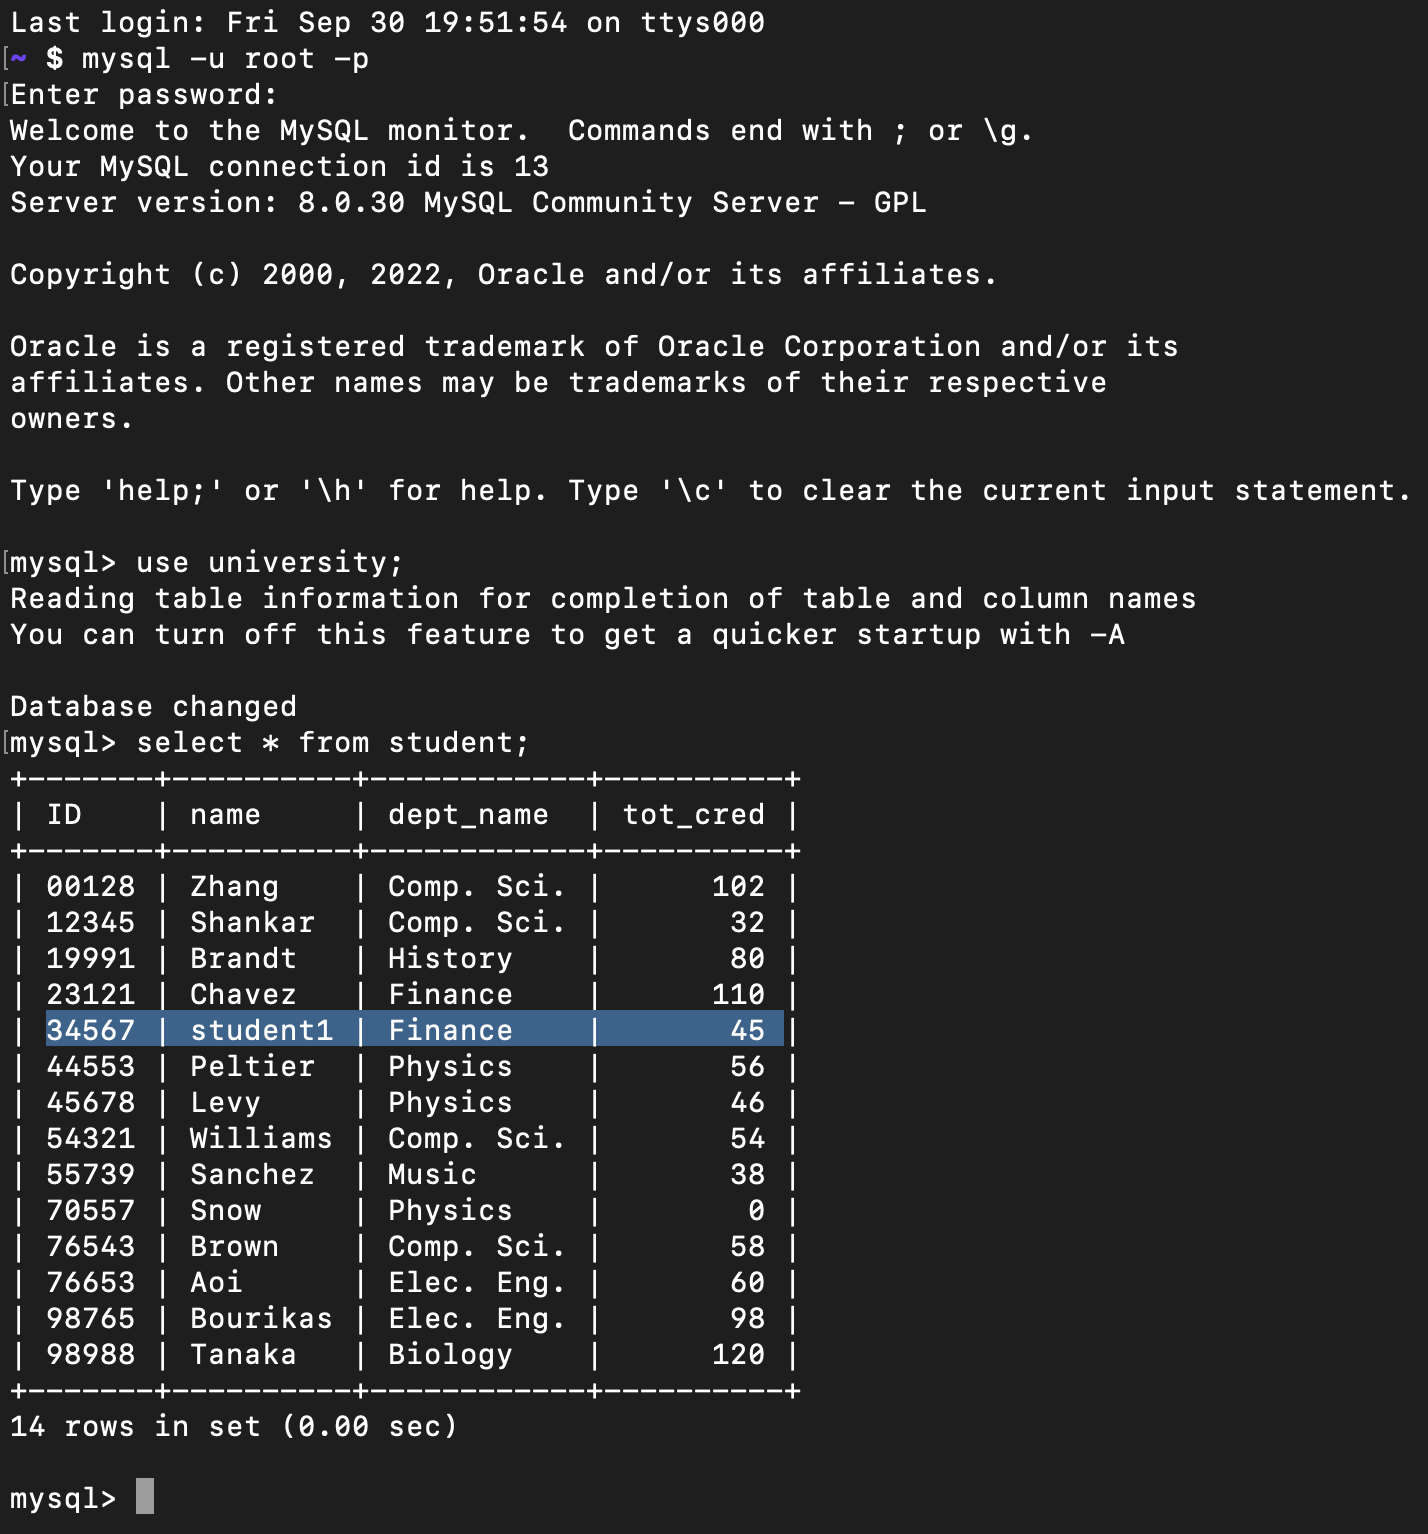
\includegraphics[scale=0.6]{screenshots/a14.png}
    \label{fig:my_label1}
    \caption{Showing the newly inserted data}
\end{figure}
\newpage

%---------------------------------------------------------------------

\section{Part B: Library Management System}

\subsection{Features of Library Management System }
\begin{itemize}
\item While adding the book, we check if the book\_id already exists, otherwise   
    add the book details to the book table using a servlet named
    AddServlet.java. Then it displays the result accordingly.
\item  While issuing the book, we add the issue details in the issue table if a       student with given student\_id and book with given book\_id exists using a        servlet named IssueServlet.java. Then it displays the result accordingly.
\end{itemize}

\subsection{Setup and Implementation}

\begin{itemize}
\item  All the program files related to part B are inside the 
    \texttt{Part\_B} directory. 
\item  For the programs related to task1 and task2 for the things like        
    creating tables and inserting data into them, can checkout the 
    \texttt{b1.sql}, \texttt{b2.sql} and \texttt{b3.sql} files. 
\item  For task3, Open the \texttt{LibraryProject} directory inside Eclipse by 
    clicking on File $\rightarrow$ Open Project From File System. After that can do the required setup.
\item  Can follow the handout given if any errors occur while setting up the 
    project.
\item  Now, after setting everything, right click on project name, then
    click Build Path $\rightarrow$ Configure build path. After that
    choose apache tomcat server and click on the Apply and Close button.
\item  To run the application, right click the project $\rightarrow$ Run as 
    $\rightarrow$ Run on server.
\item Once the server is up, access the following URL:    
\end{itemize}

\vspace{-2mm}

{\centerline{\underline{http://localhost:8080/LibraryProject/Home.jsp}}}

\newpage

\subsection{Task 1: Designing the database Library and creating tables.}

\subsubsection*{Query}
\fbox{ 
    \begin{minipage}{40em}
    \inputminted{mysql}{src/b1.sql}
    \end{minipage}
}

\subsubsection*{Result}
\begin{figure}[!hbt]
    \centering
    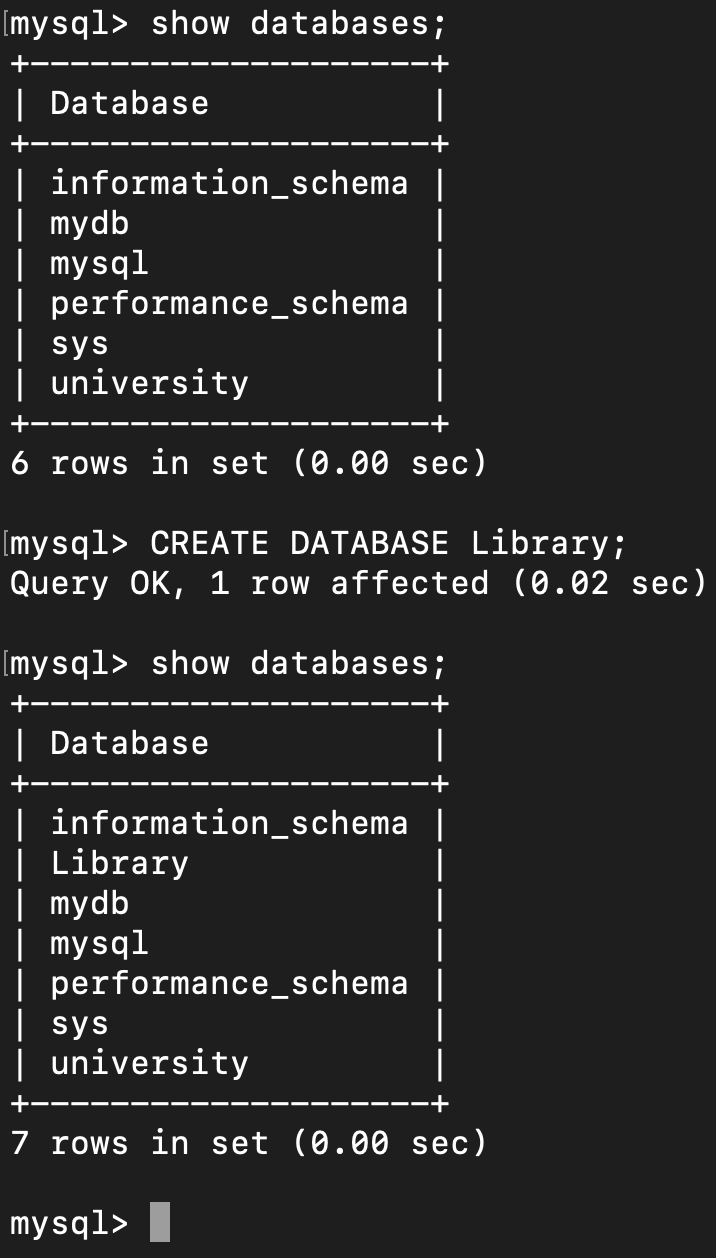
\includegraphics[scale=0.7]{screenshots/b1_01.png}
    \label{fig:my_label1}
    \caption{Creation of new Library database}
\end{figure}

\newpage

\subsubsection*{Query}
\fbox{ 
    \begin{minipage}{40em}
    \inputminted{mysql}{src/b2.sql}
    \end{minipage}
}

\newpage

\subsubsection*{Result}
\begin{figure}[!hbt]
    \centering
    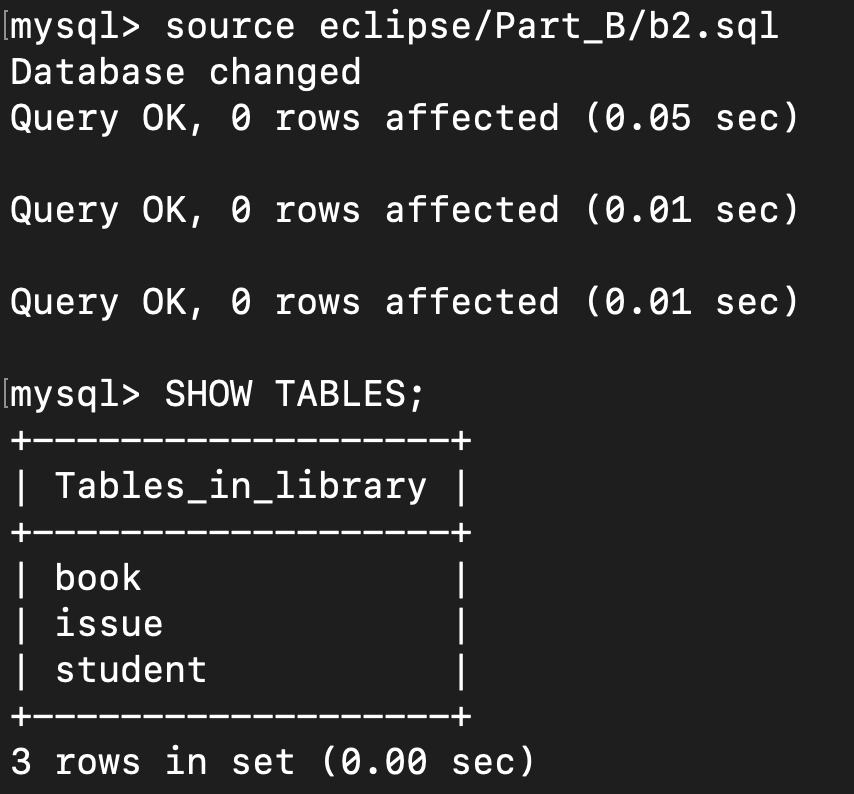
\includegraphics[scale=0.8]{screenshots/b1_02.png}
    \label{fig:my_label1}
    \caption{Creation of tables inside Library database}
\end{figure}

\newpage

%-------------------------------------------------------------------

\subsection{Task 2: Loading data into the tables}

\subsubsection{Query}
\fbox{ 
    \begin{minipage}{40em}
    \inputminted{mysql}{src/b3.sql}
    \end{minipage}
}

\newpage

\subsubsection{Results}
\begin{figure}[!hbt]
    \centering
    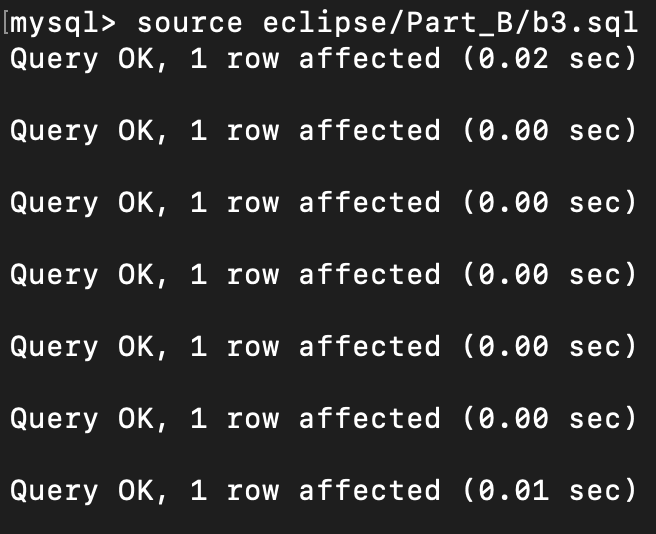
\includegraphics[scale=1.1]{screenshots/b2_01.png}
    \label{fig:my_label1}
    \caption{Insertion of data into those tables}
\end{figure}

\begin{figure}[!hbt]
    \centering
    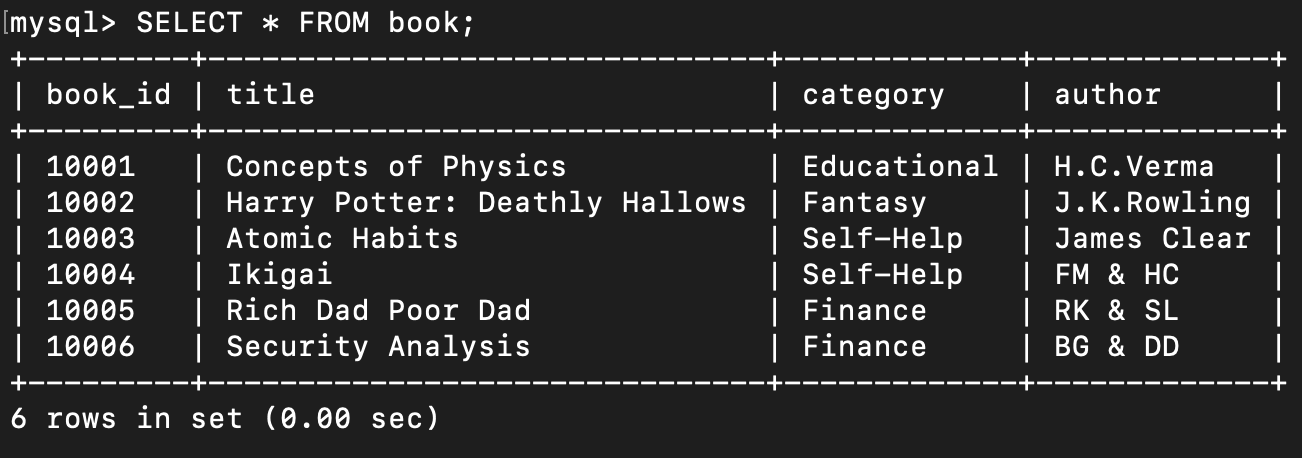
\includegraphics[scale=0.75]{screenshots/b2_02.png}
    \label{fig:my_label1}
    \caption{Book table}
\end{figure}

\newpage

\begin{figure}[!hbt]
    \centering
    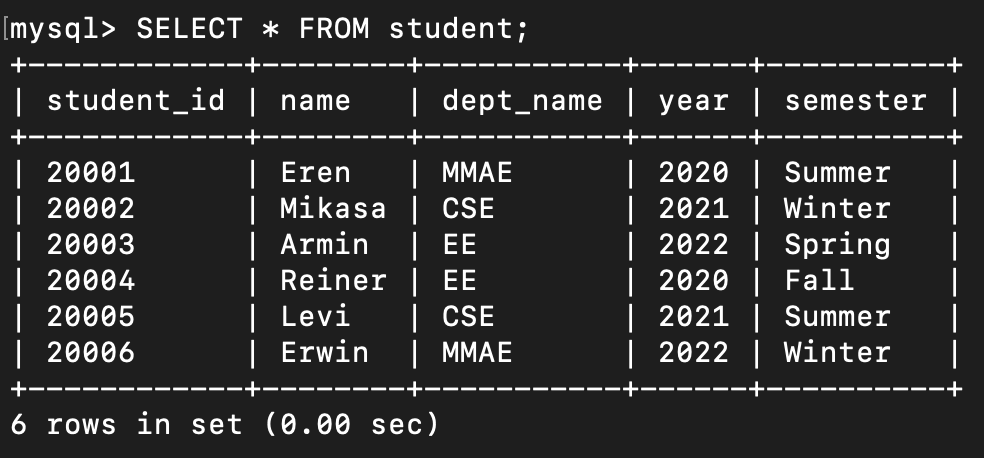
\includegraphics[scale=0.9]{screenshots/b2_03.png}
    \label{fig:my_label1}
    \caption{Student table}
\end{figure}

\begin{figure}[!hbt]
    \centering
    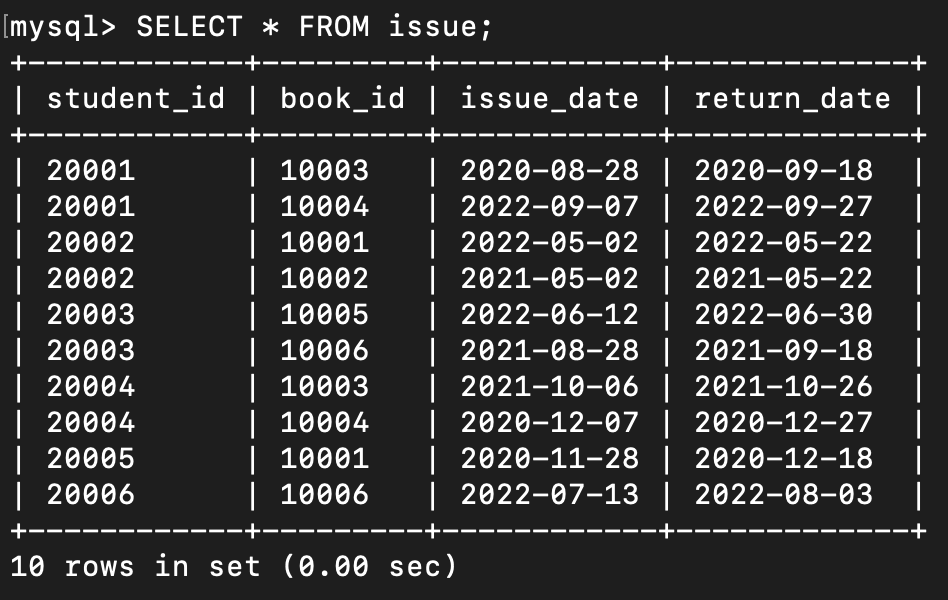
\includegraphics[scale=0.9]{screenshots/b2_04.png}
    \label{fig:my_label1}
    \caption{Issue table}
\end{figure}

\newpage

%-------------------------------------------------------------------

\subsection{Task 3: Creating a Java-J2EE project}

\subsubsection{Workspace Screenshots}

\begin{figure}[!hbt]
    \centering
    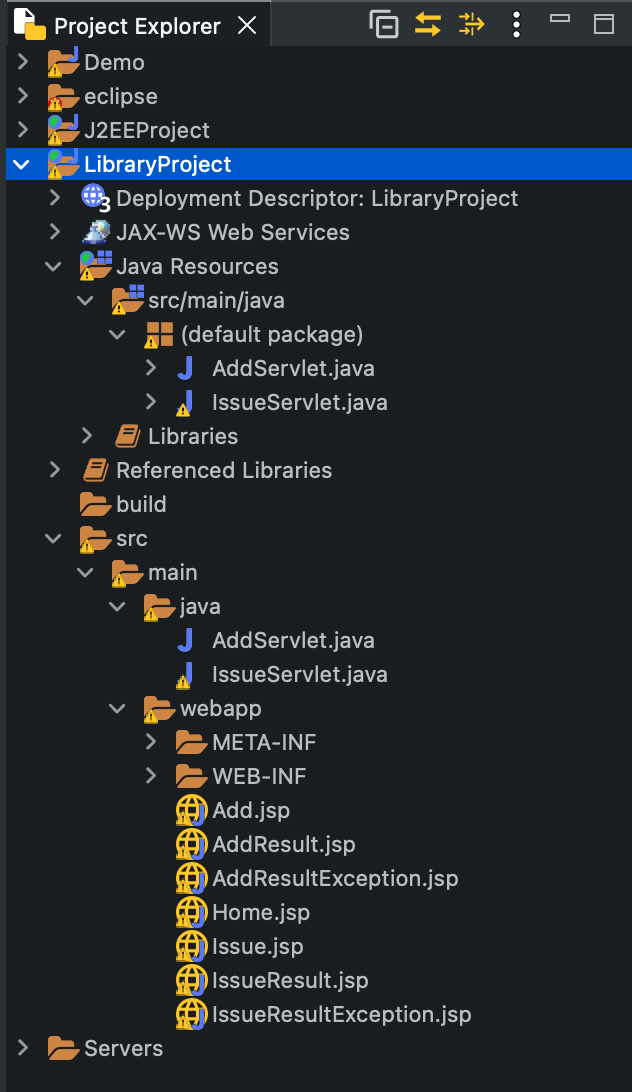
\includegraphics[scale=0.33]{screenshots/b3_01.png}
    \label{fig:my_label1}
    \caption{Workspace directory files}
\end{figure}

\begin{figure}[!hbt]
    \centering
    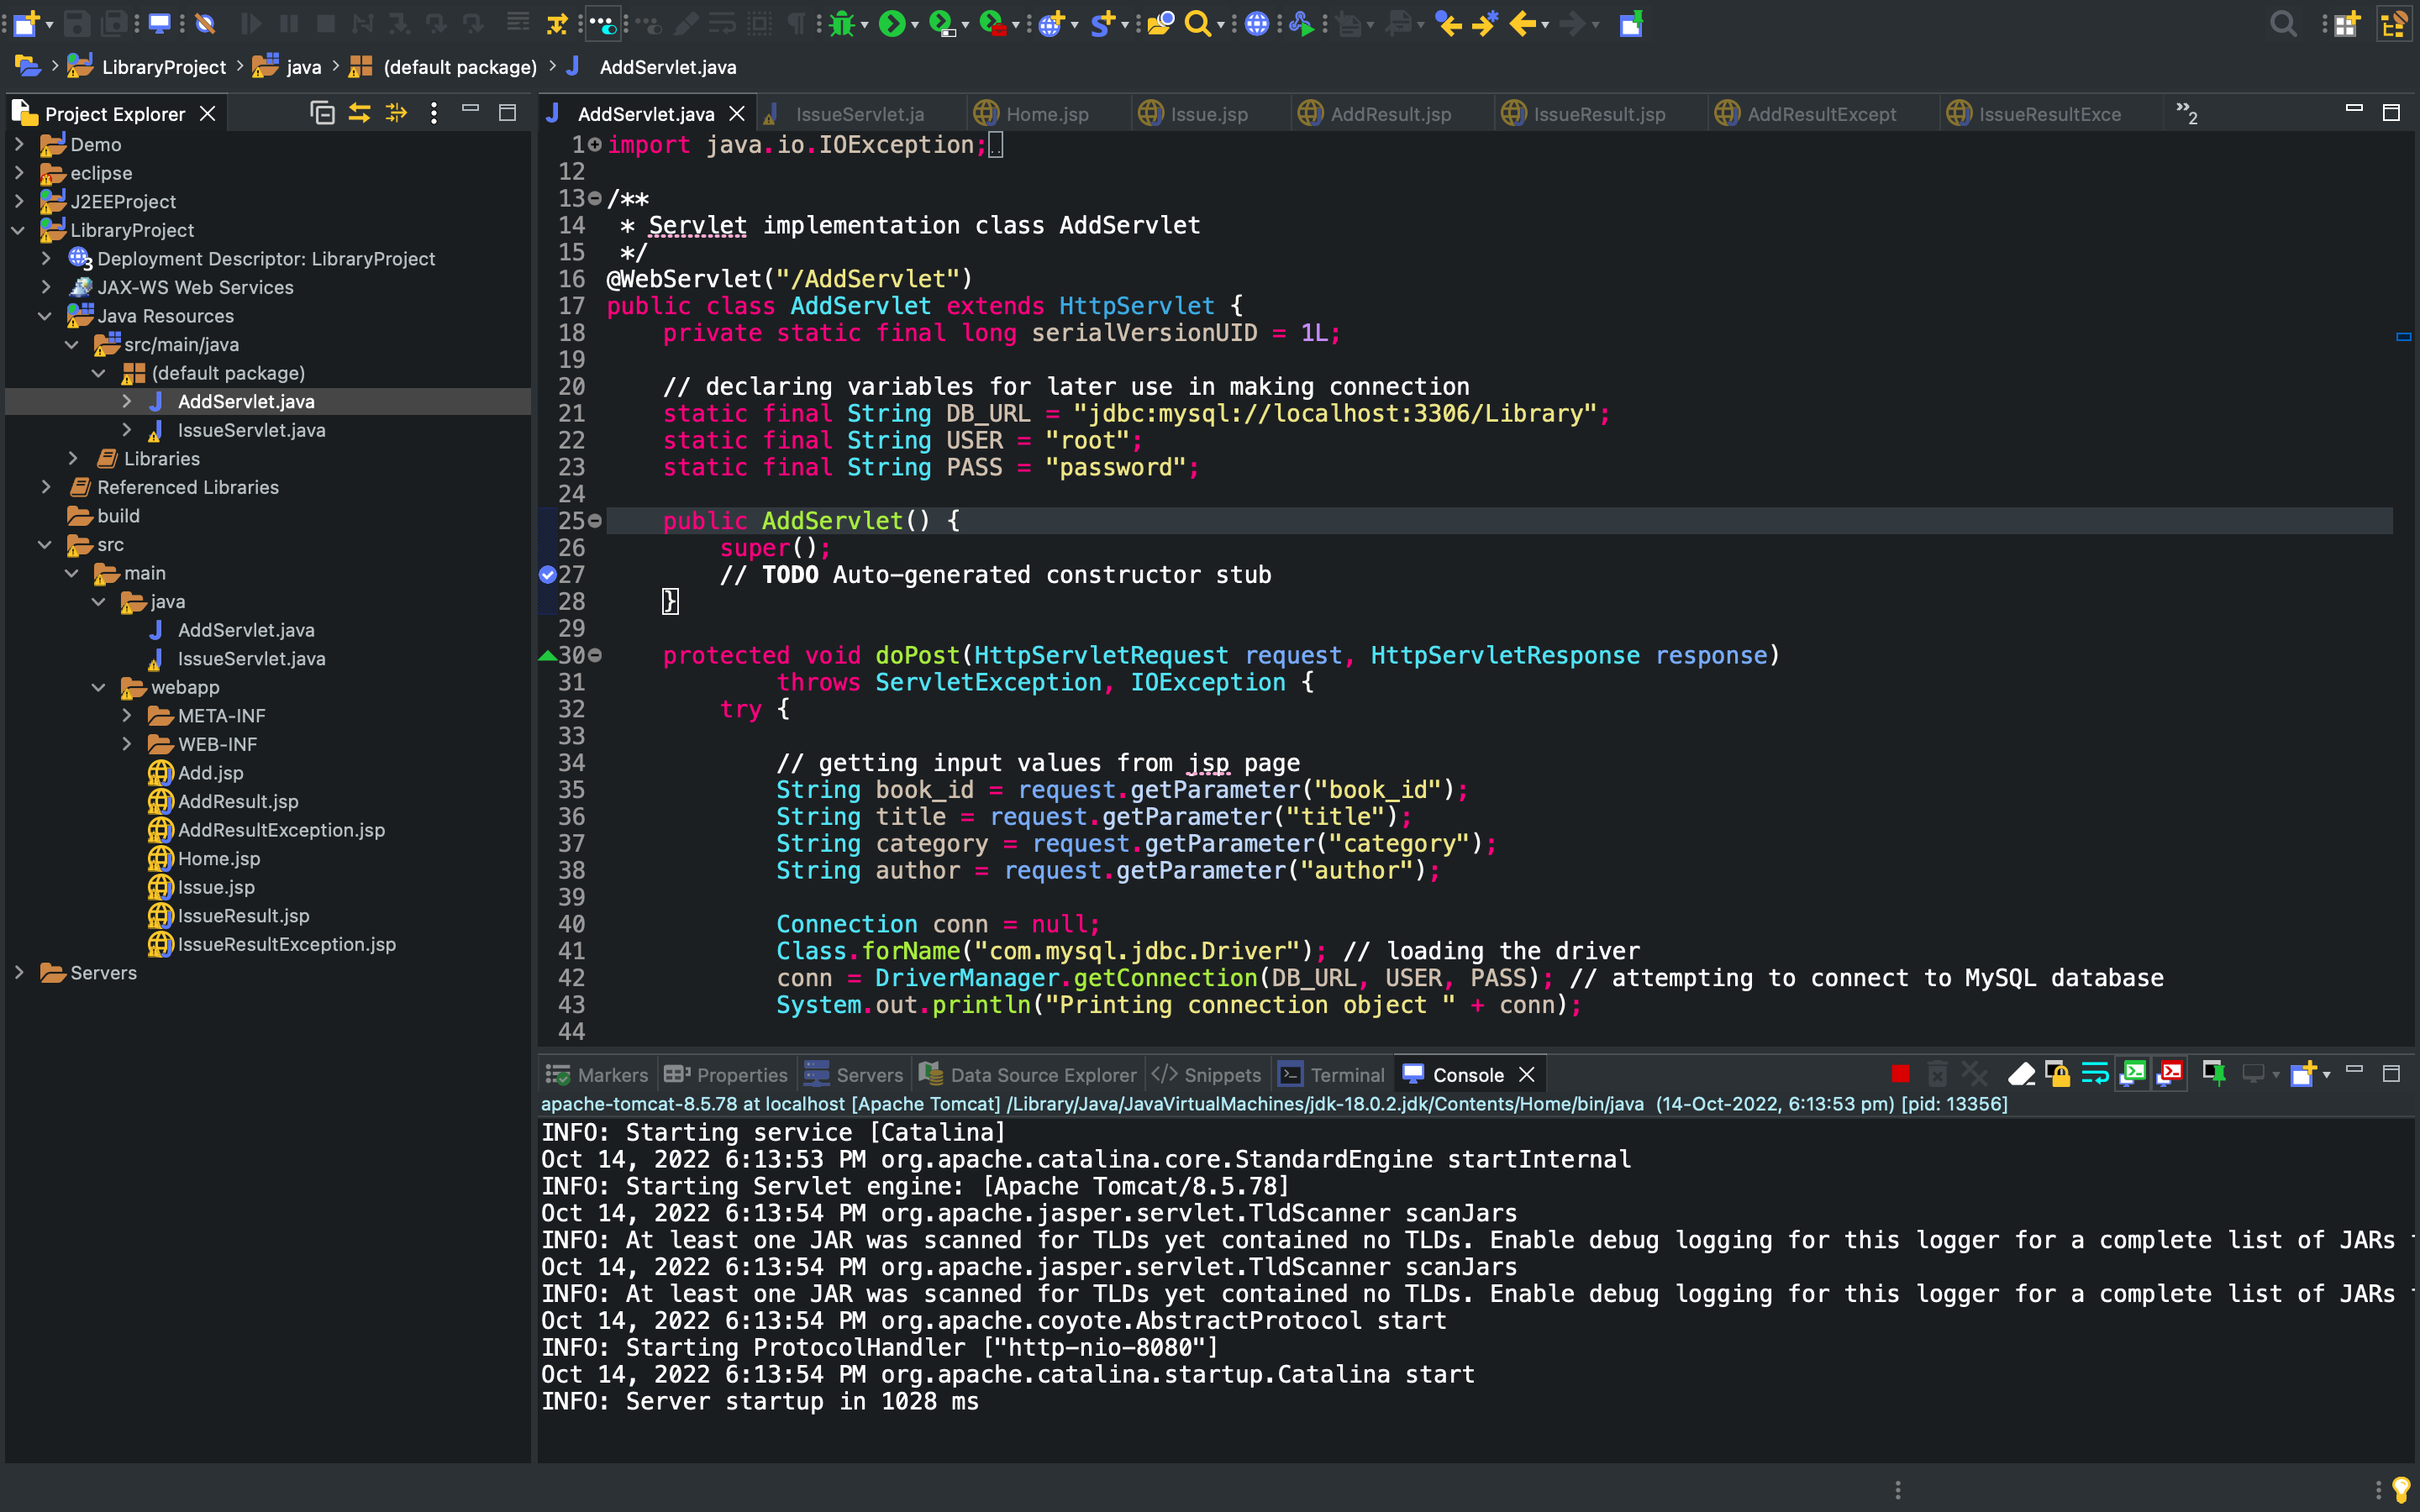
\includegraphics[scale=0.32]{screenshots/b3_02.png}
    \label{fig:my_label1}
    \caption{Workspace screen with running server}
\end{figure}

\newpage

\subsubsection{View of webpages created}

\begin{figure}[!hbt]
    \centering
    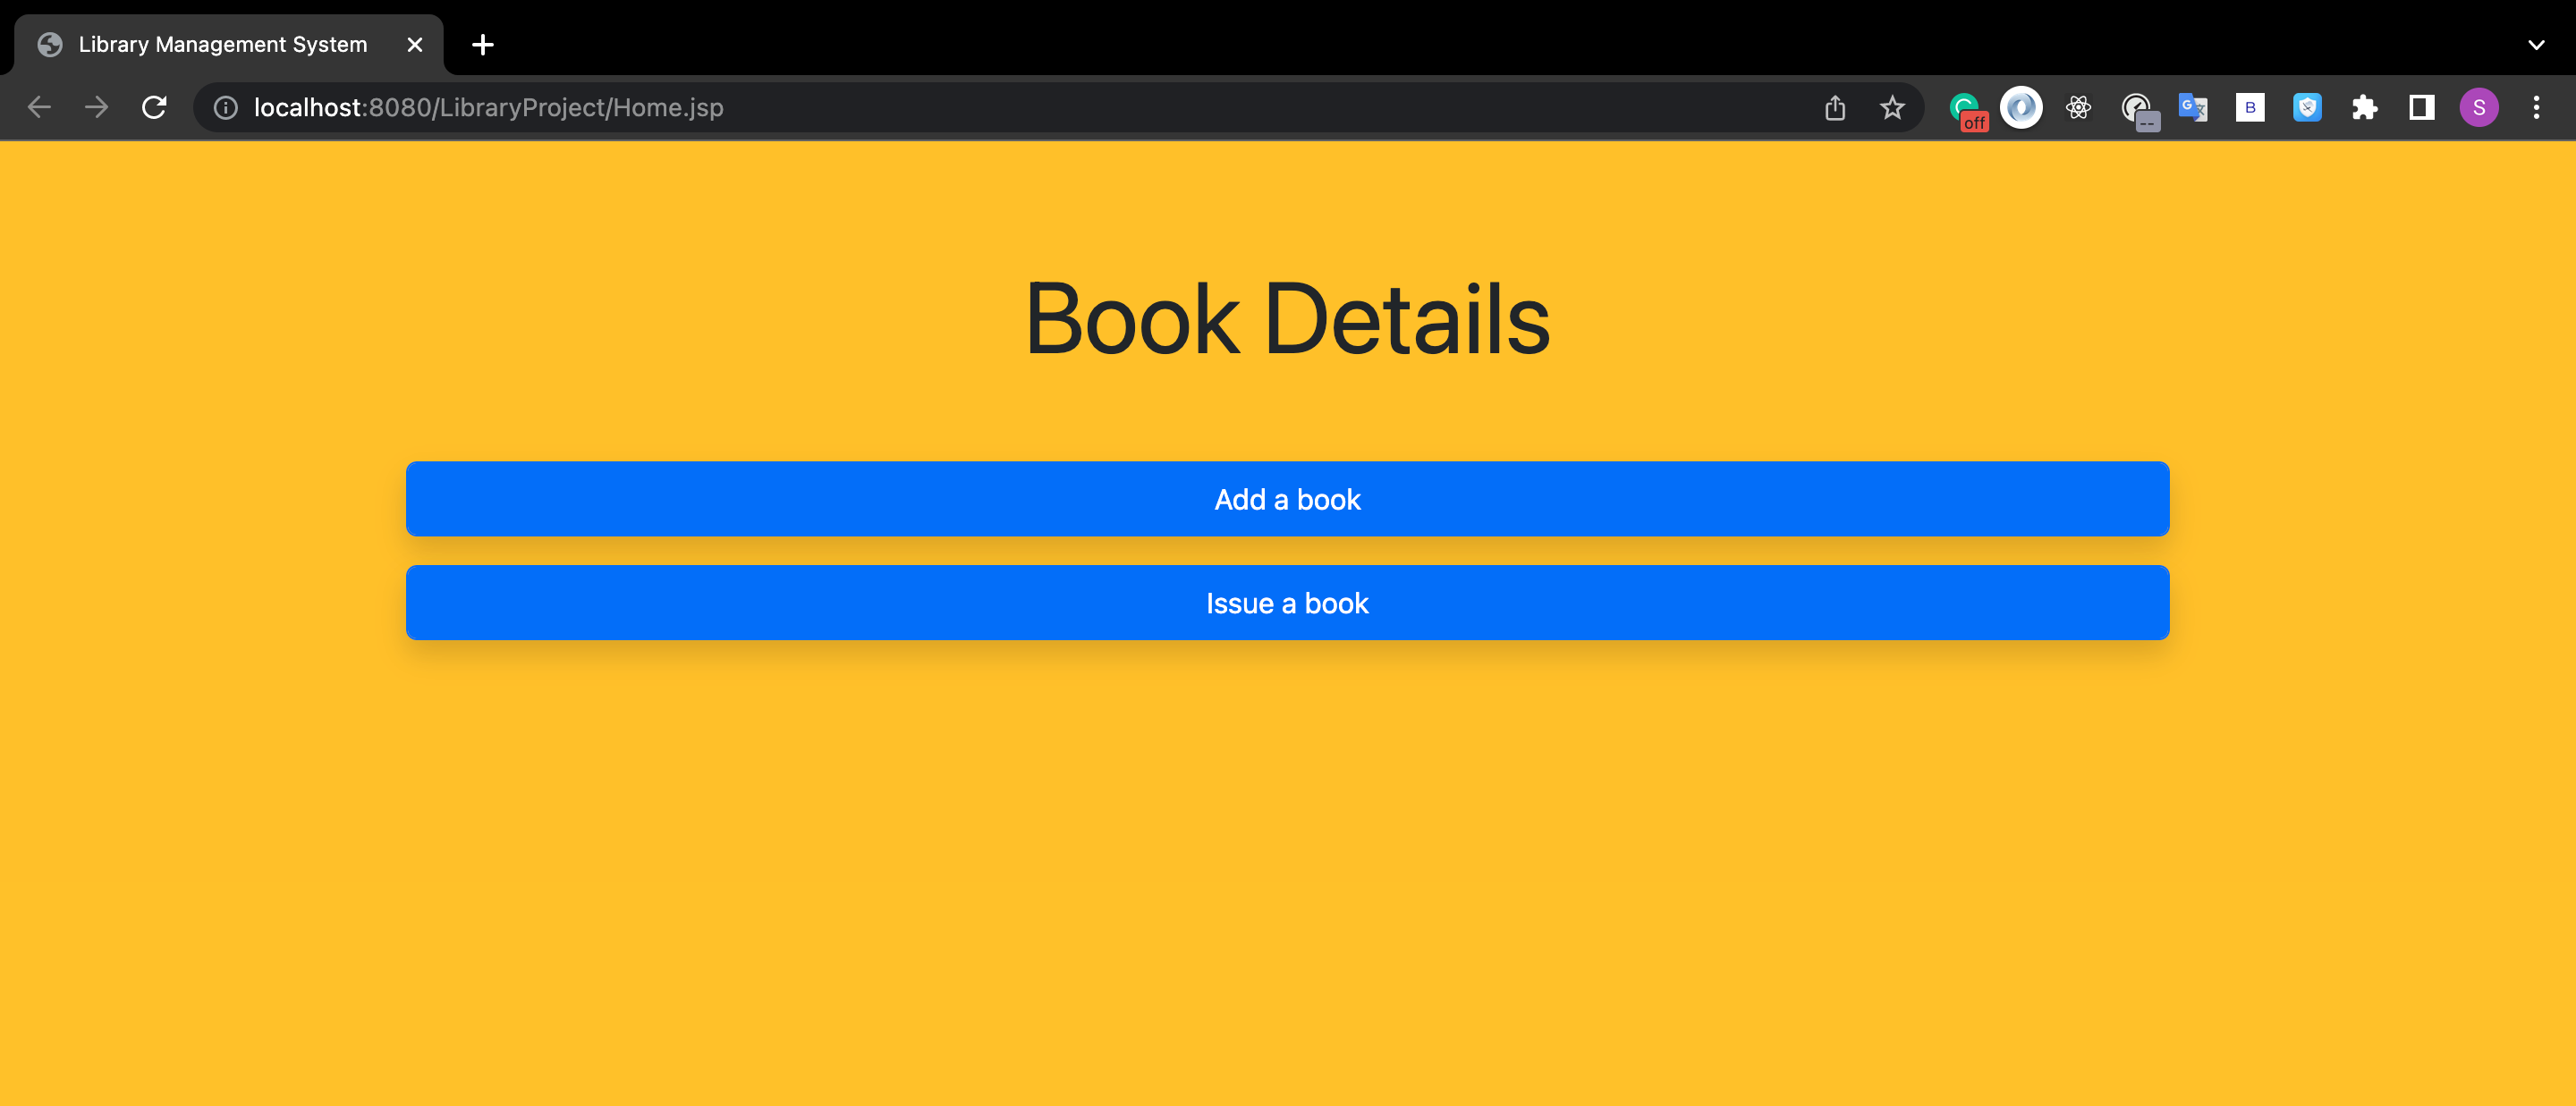
\includegraphics[scale=0.34]{screenshots/b3_ 03.png}
    \label{fig:my_label1}
    \caption{Home.jsp}
\end{figure}

\begin{figure}[!hbt]
    \centering
    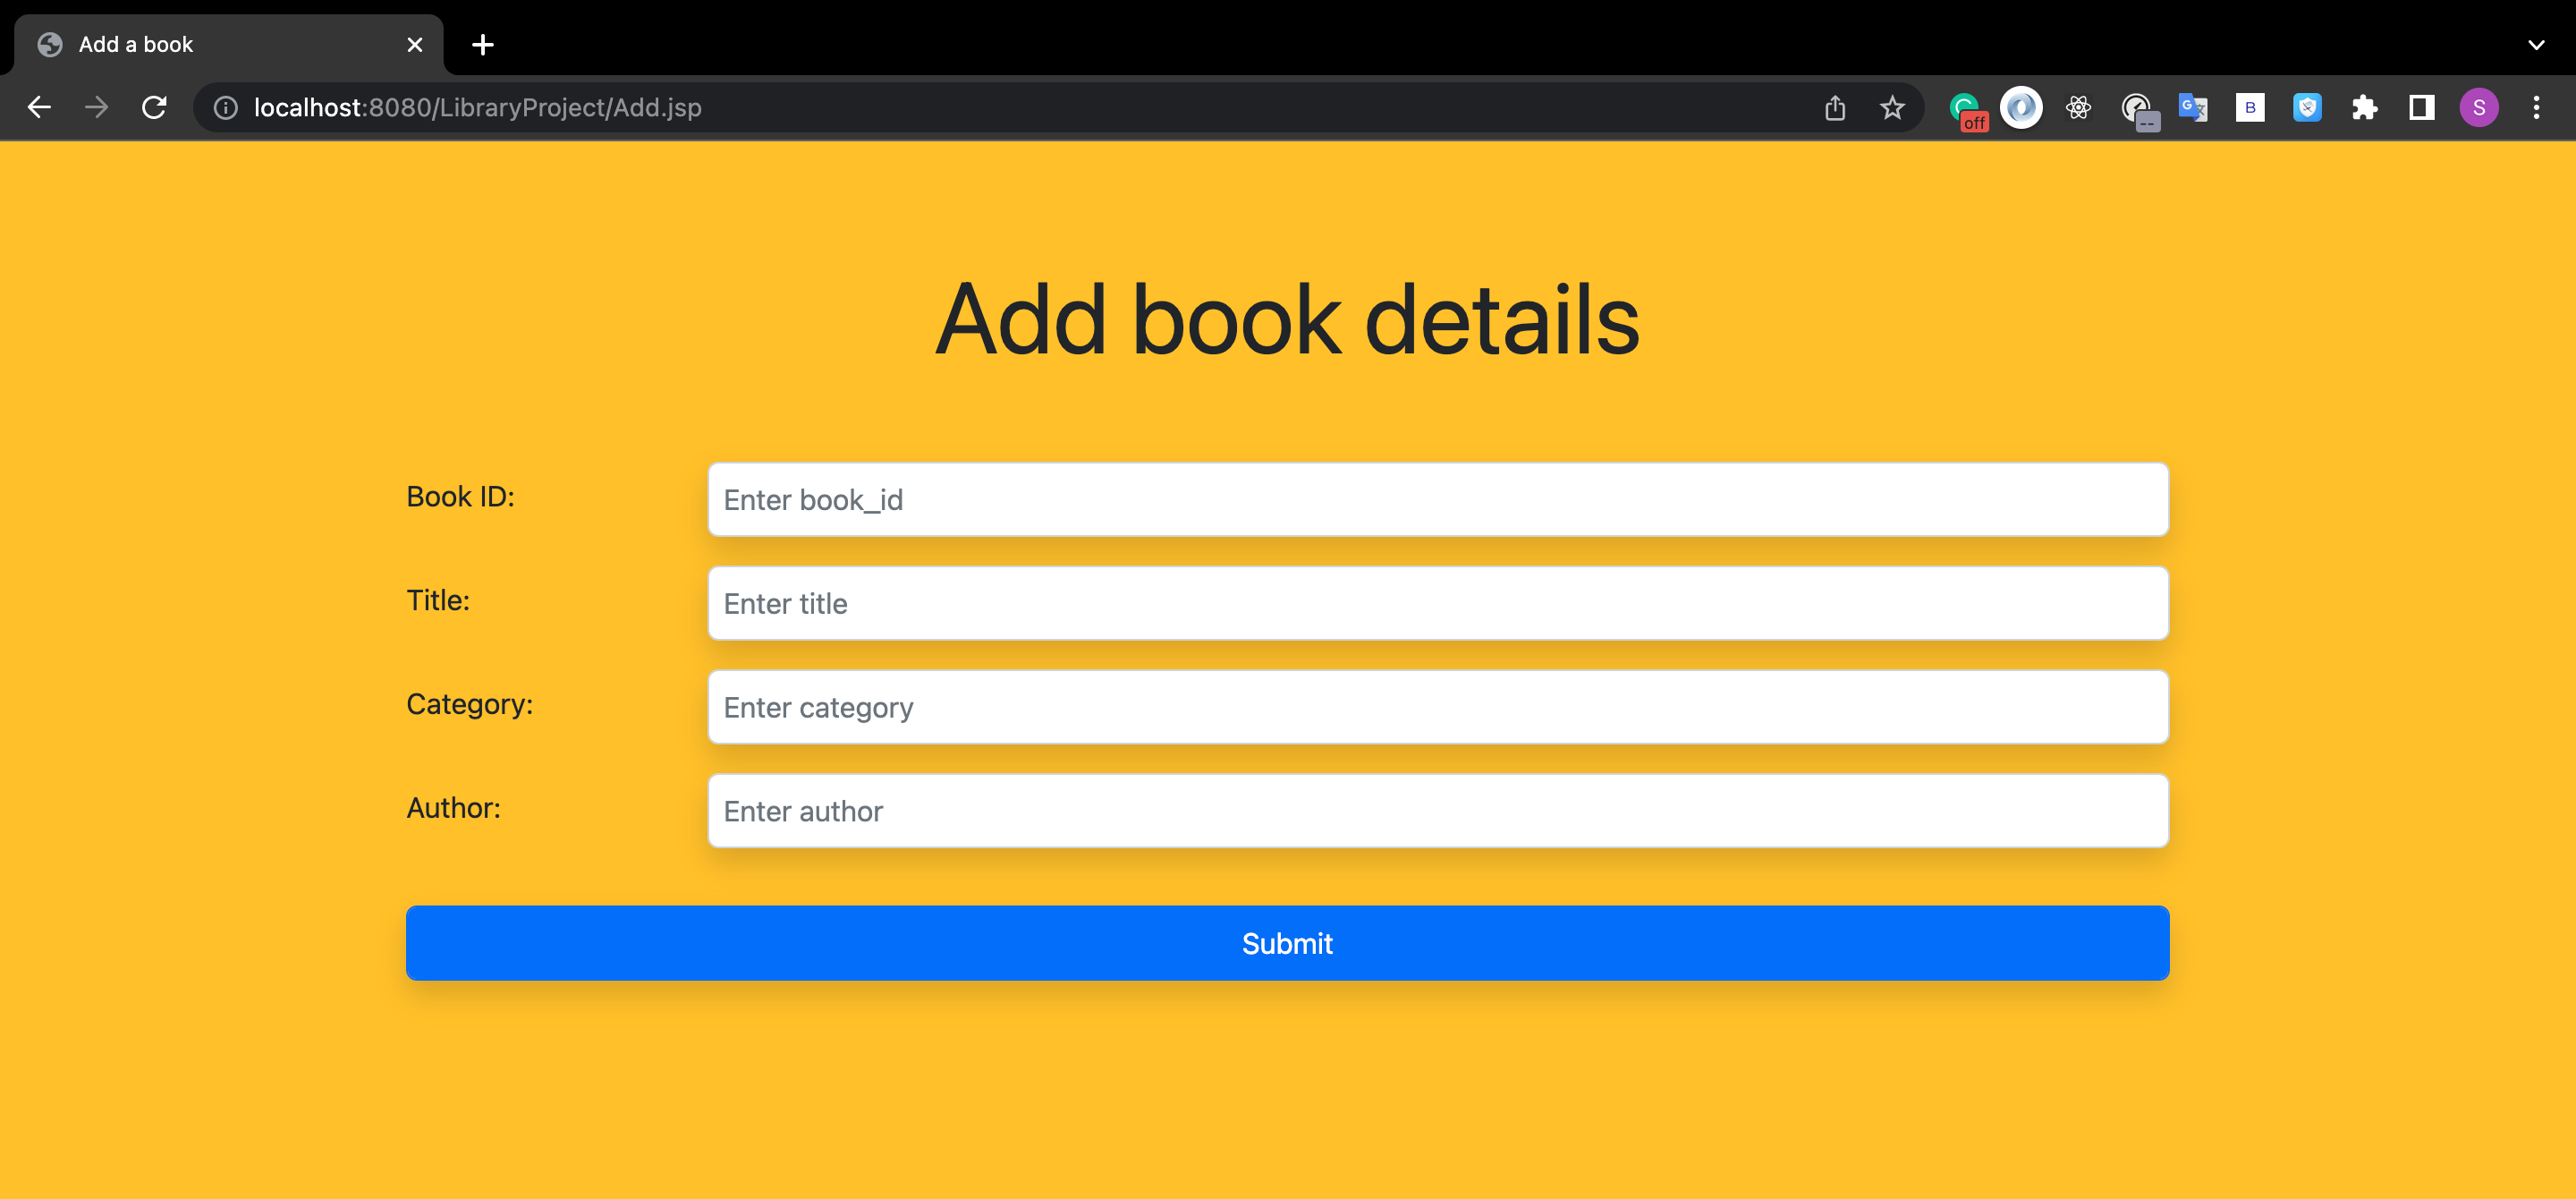
\includegraphics[scale=0.34]{screenshots/b3_04.png}
    \label{fig:my_label1}
    \caption{Add.jsp}
\end{figure}

\newpage

\begin{figure}[!hbt]
    \centering
    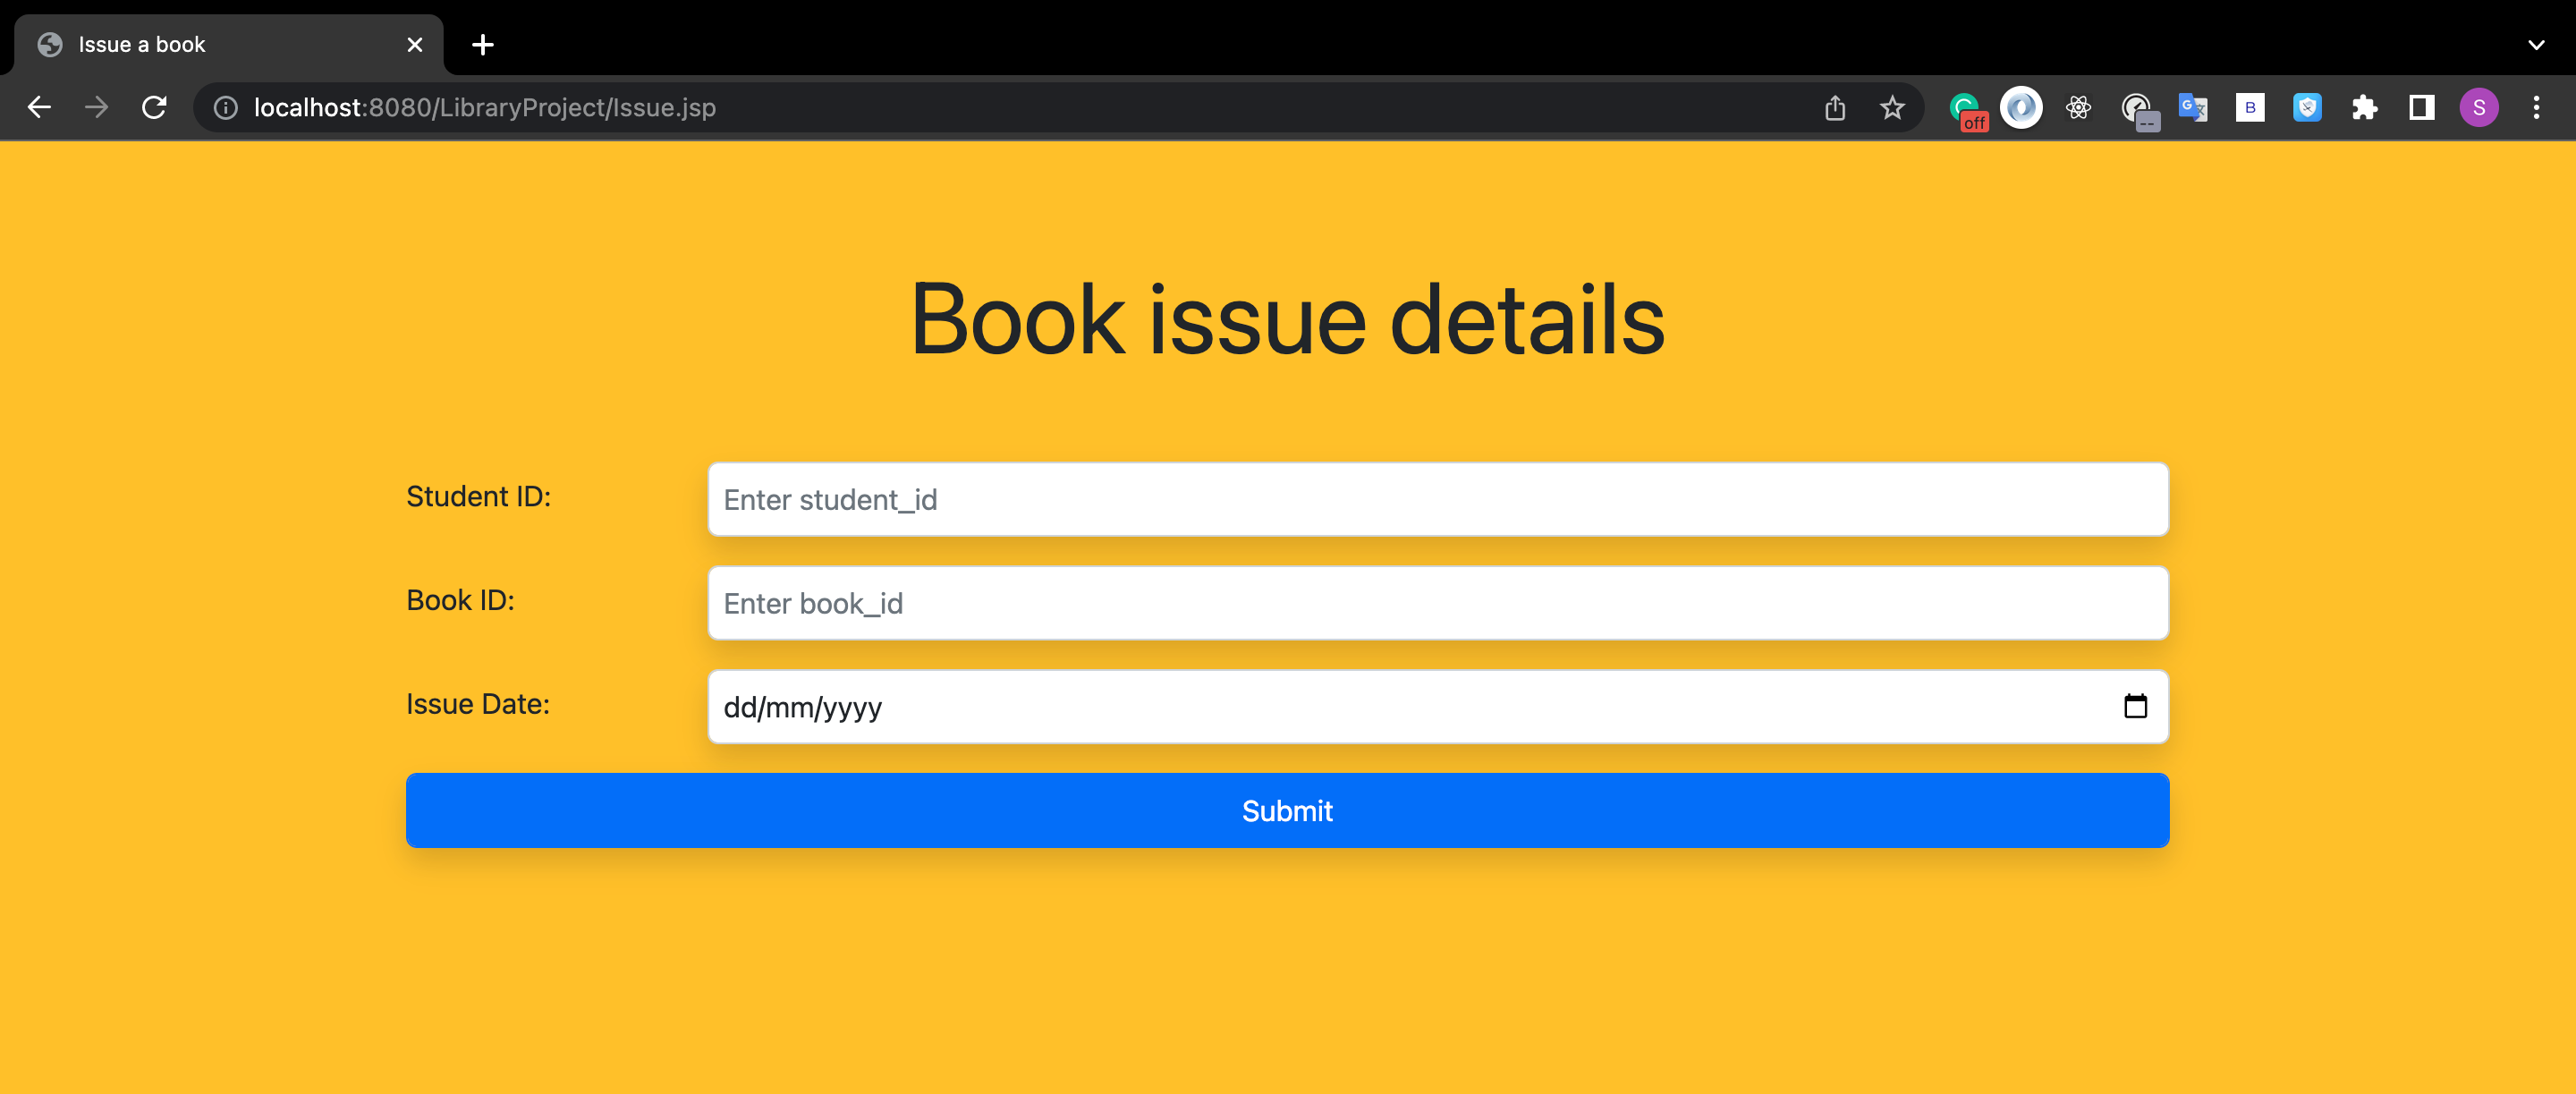
\includegraphics[scale=0.34]{screenshots/b3_05.png}
    \label{fig:my_label1}
    \caption{Issue.jsp}
\end{figure}

\newpage

\subsubsection{Adding a book}

\begin{figure}[!hbt]
    \centering
    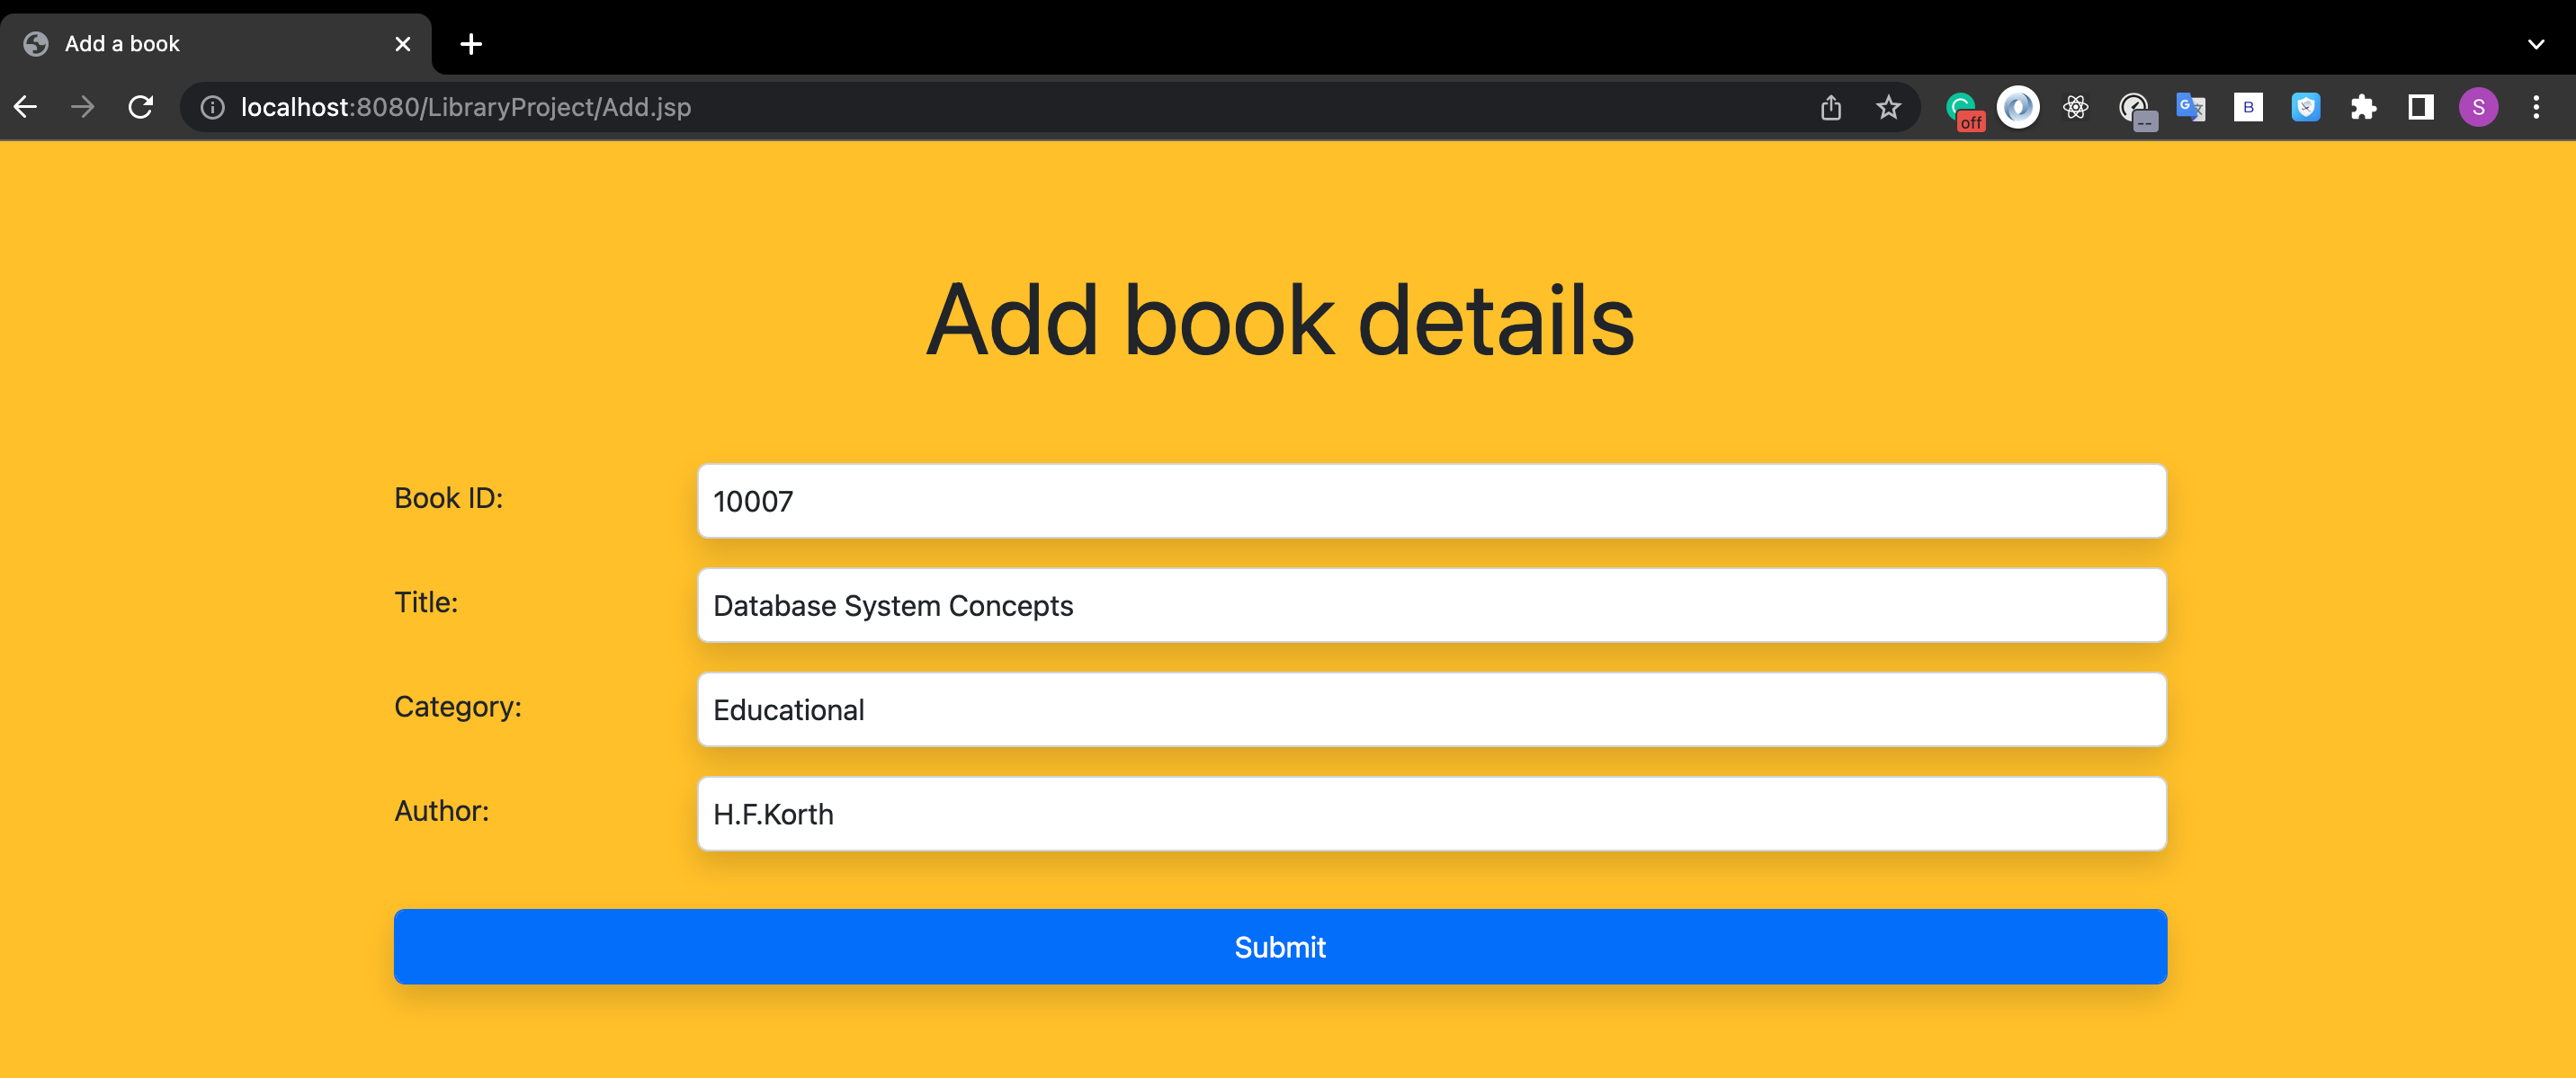
\includegraphics[scale=0.34]{screenshots/b3_06.png}
    \label{fig:my_label1}
    \caption{Add.jsp with the inputs}
\end{figure}

\begin{figure}[!hbt]
    \centering
    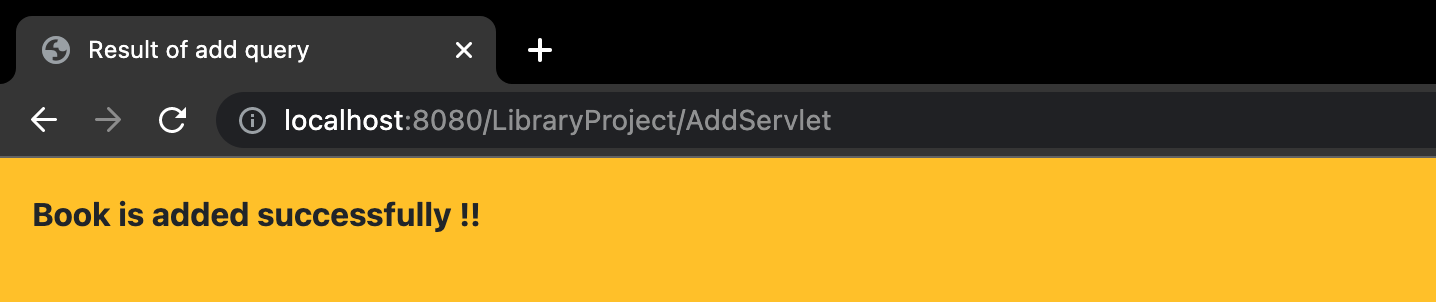
\includegraphics[scale=0.5]{screenshots/b3_07.png}
    \label{fig:my_label1}
    \caption{AddResult.jsp with successful insertion of add query}
\end{figure}

\begin{figure}[!hbt]
    \centering
    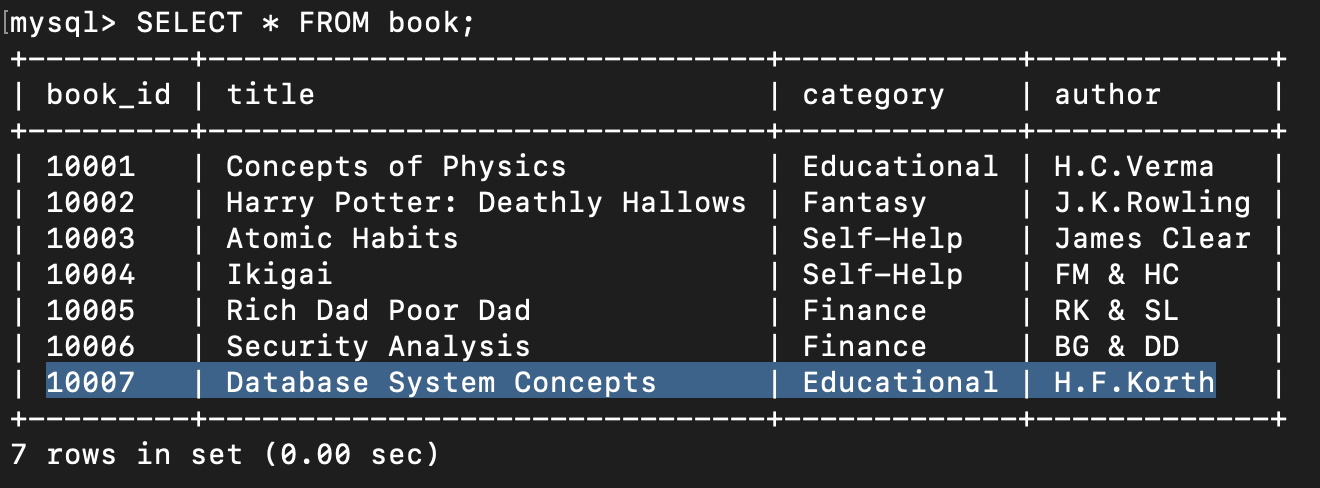
\includegraphics[scale=0.61]{screenshots/b3_08.png}
    \label{fig:my_label1}
    \caption{Updated \oldtexttt{book} table}
\end{figure}

\newpage

\subsubsection{Issuing a book}

\begin{figure}[!hbt]
    \centering
    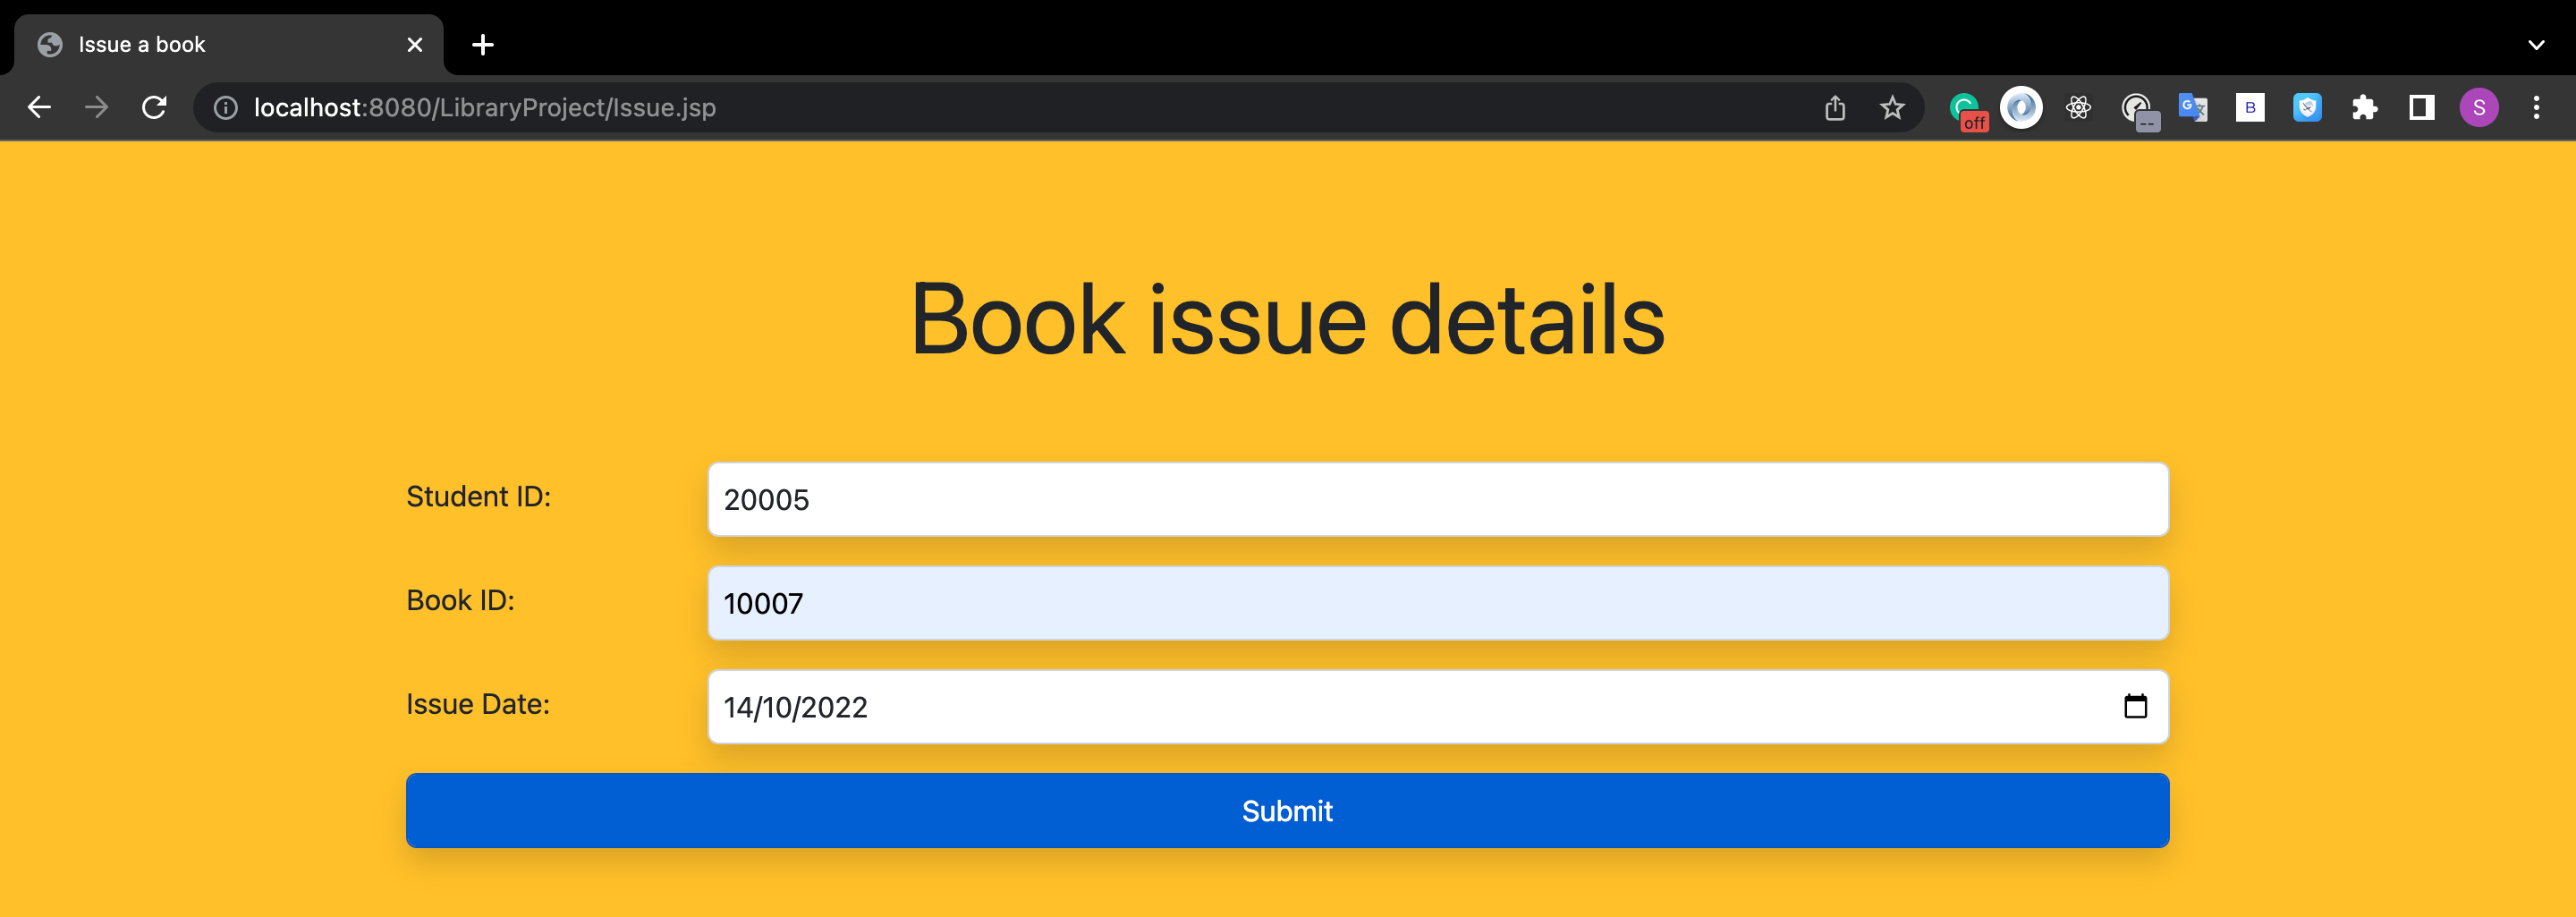
\includegraphics[scale=0.34]{screenshots/b3_09.png}
    \label{fig:my_label1}
    \caption{Issue.jsp with the inputs}
\end{figure}

\begin{figure}[!hbt]
    \centering
    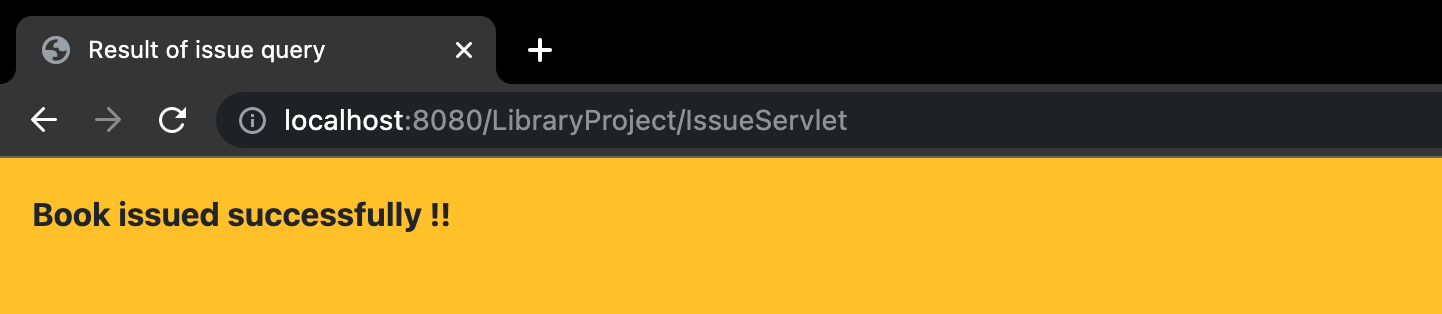
\includegraphics[scale=0.47]{screenshots/b3_10.png}
    \label{fig:my_label1}
    \caption{IssueResult.jsp with successful execution of issue query}
\end{figure}

\begin{figure}[!hbt]
    \centering
    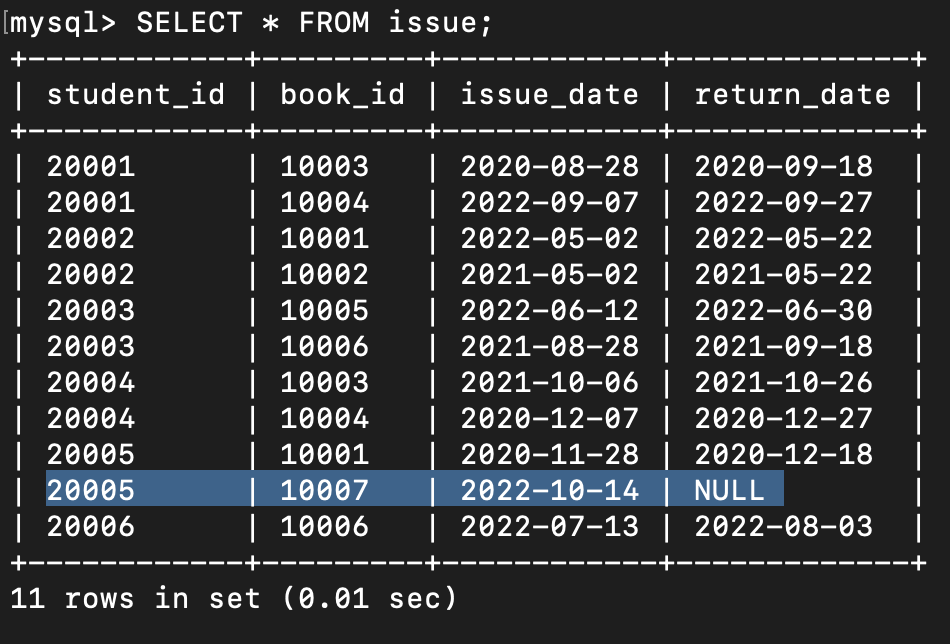
\includegraphics[scale=0.56]{screenshots/b3_11.png}
    \label{fig:my_label1}
    \caption{Updated \oldtexttt{issue} table}
\end{figure}

\newpage

\subsubsection{Adding the book with existing book\_id}

\begin{figure}[!hbt]
    \centering
    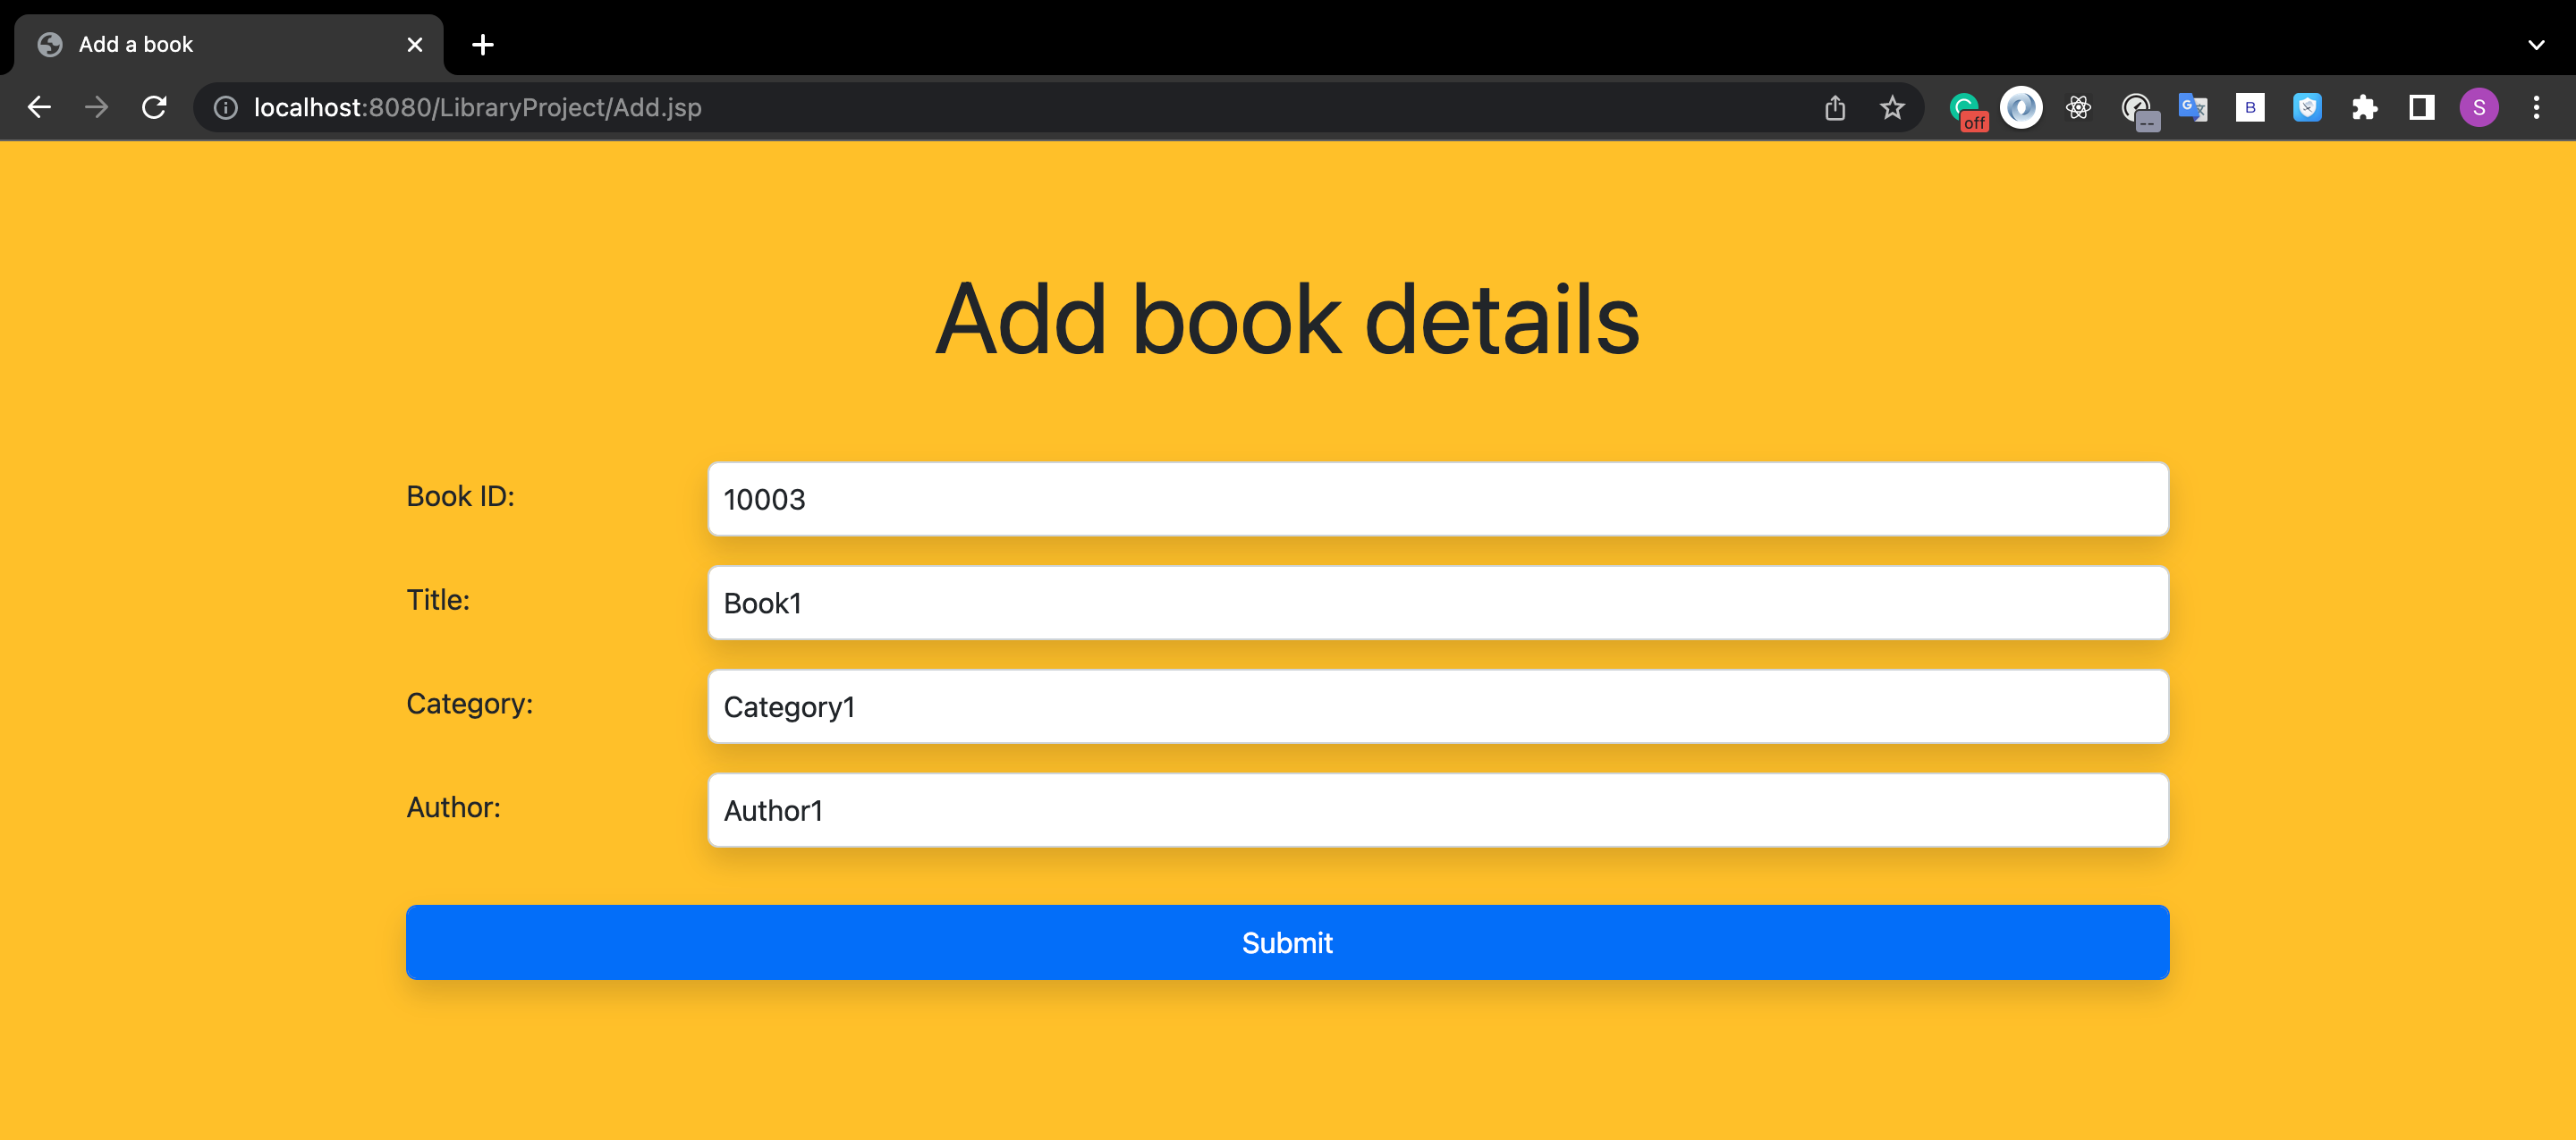
\includegraphics[scale=0.34]{screenshots/b3_12.png}
    \label{fig:my_label1}
    \caption{Add.jsp with the inputs}
\end{figure}
\vspace{2cm}
\begin{figure}[!hbt]
    \centering
    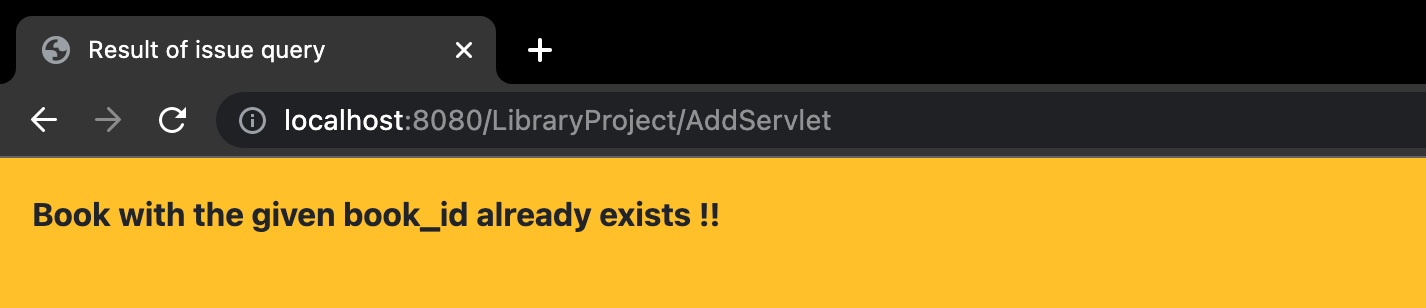
\includegraphics[scale=0.69]{screenshots/b3_13.png}
    \label{fig:my_label1}
    \caption{AddResultException.jsp with result of add query}
\end{figure}

\newpage

\subsubsection{Issuing a book with incorrect student\_id}

\begin{figure}[!hbt]
    \centering
    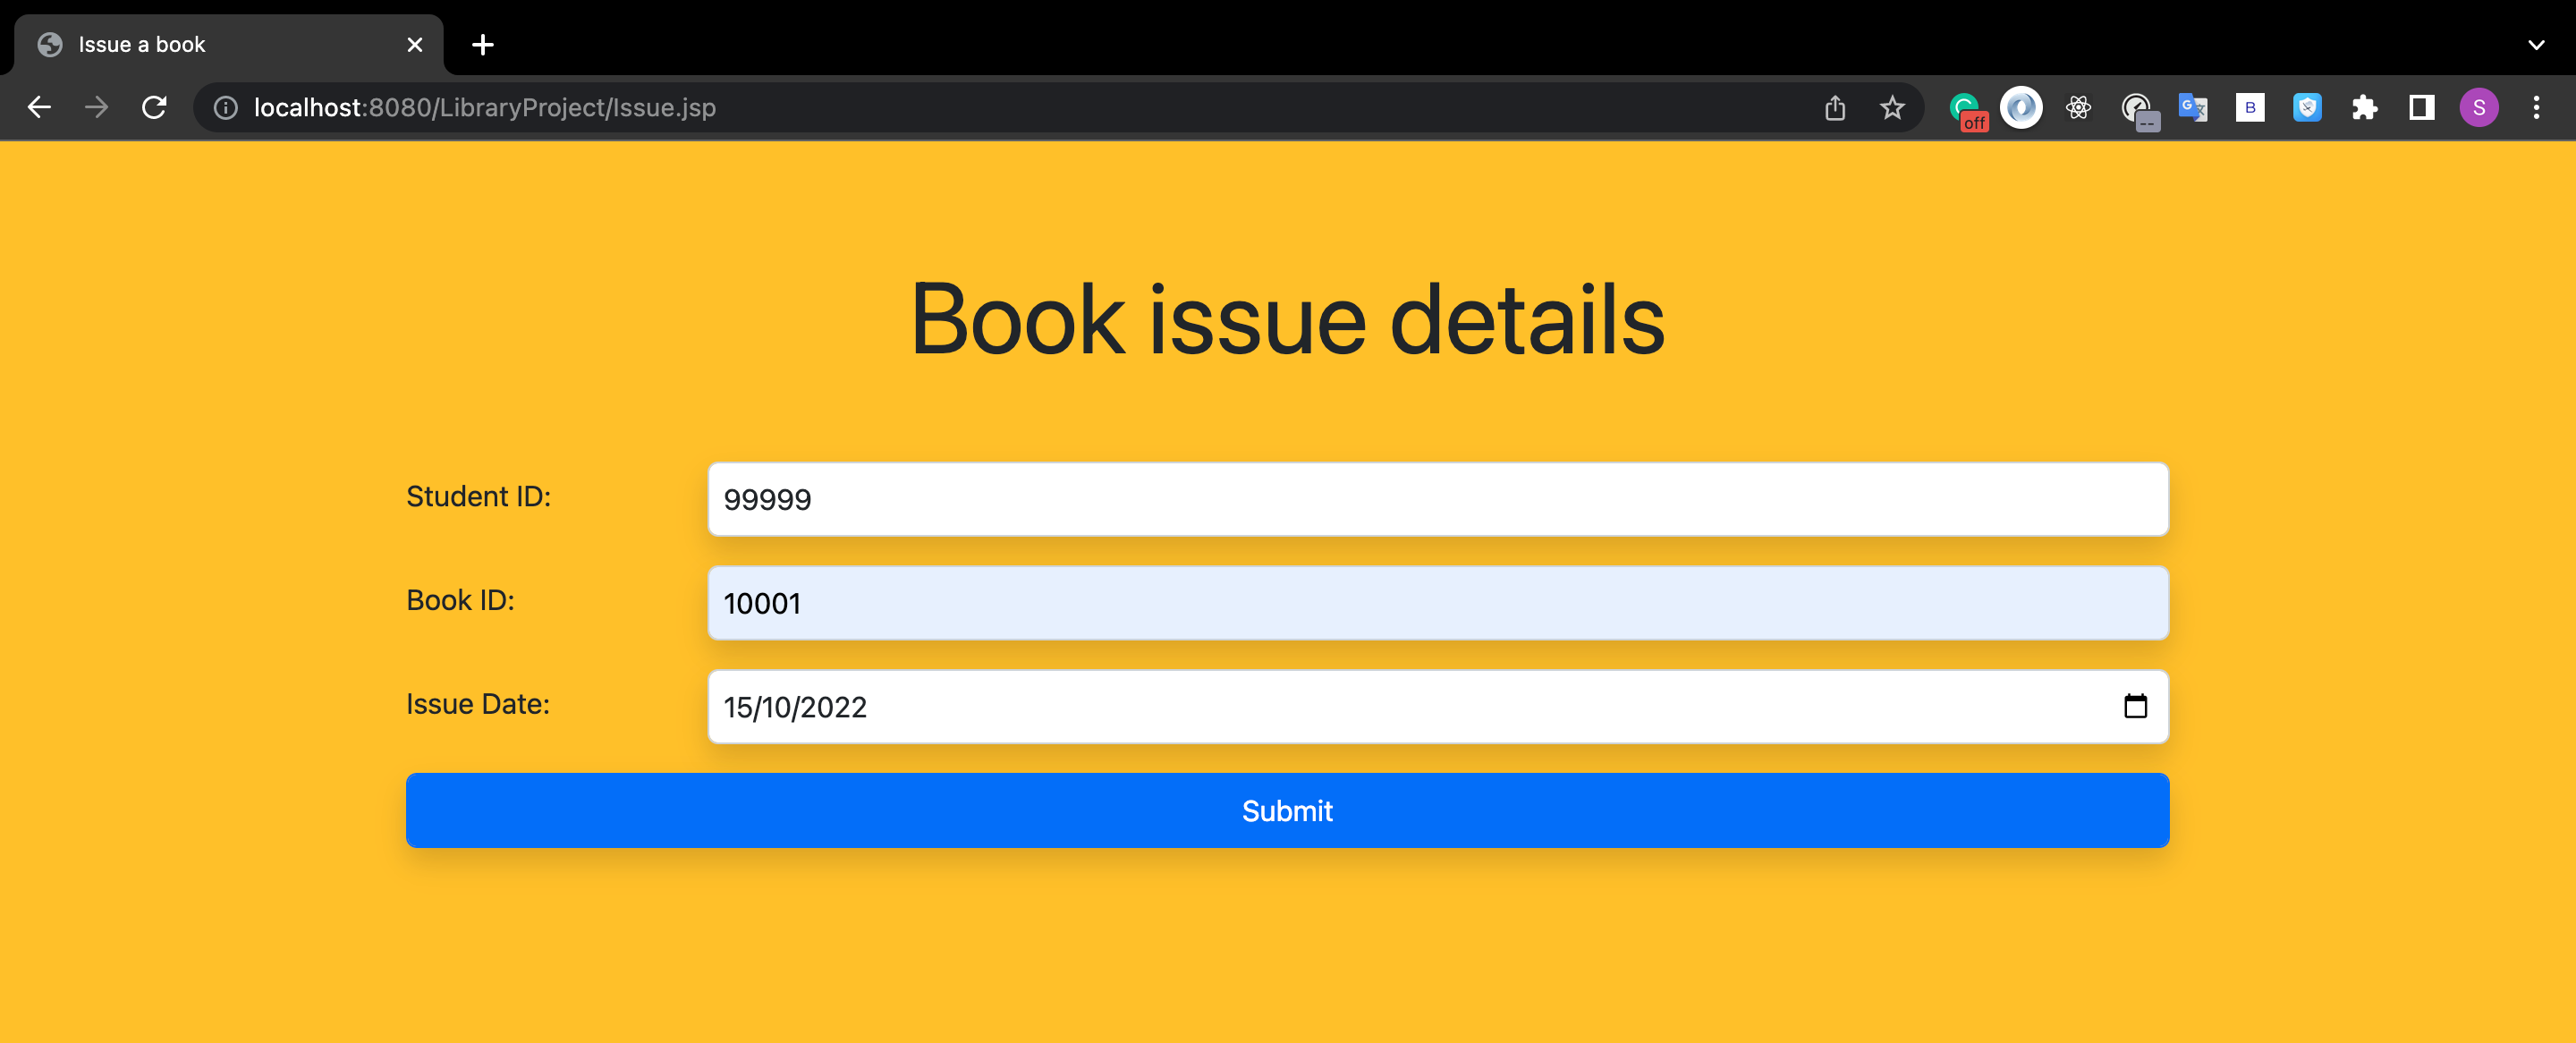
\includegraphics[scale=0.34]{screenshots/b3_14.png}
    \label{fig:my_label1}
    \caption{Issue.jsp with the inputs}
\end{figure}
\vspace{2cm}
\begin{figure}[!hbt]
    \centering
    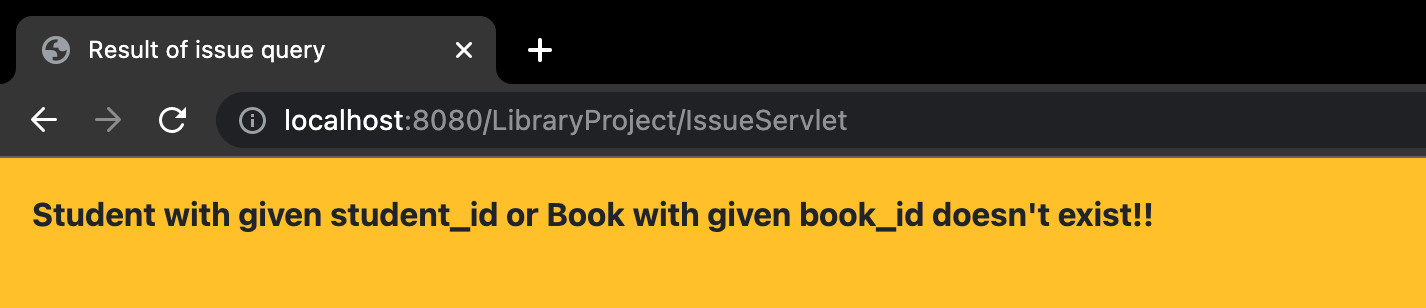
\includegraphics[scale=0.69]{screenshots/b3_15.png}
    \label{fig:my_label1}
    \caption{IssueResultException.jsp with result of issue query}
\end{figure}

\newpage

\subsubsection{Issuing a book with incorrect book\_id}

\begin{figure}[!hbt]
    \centering
    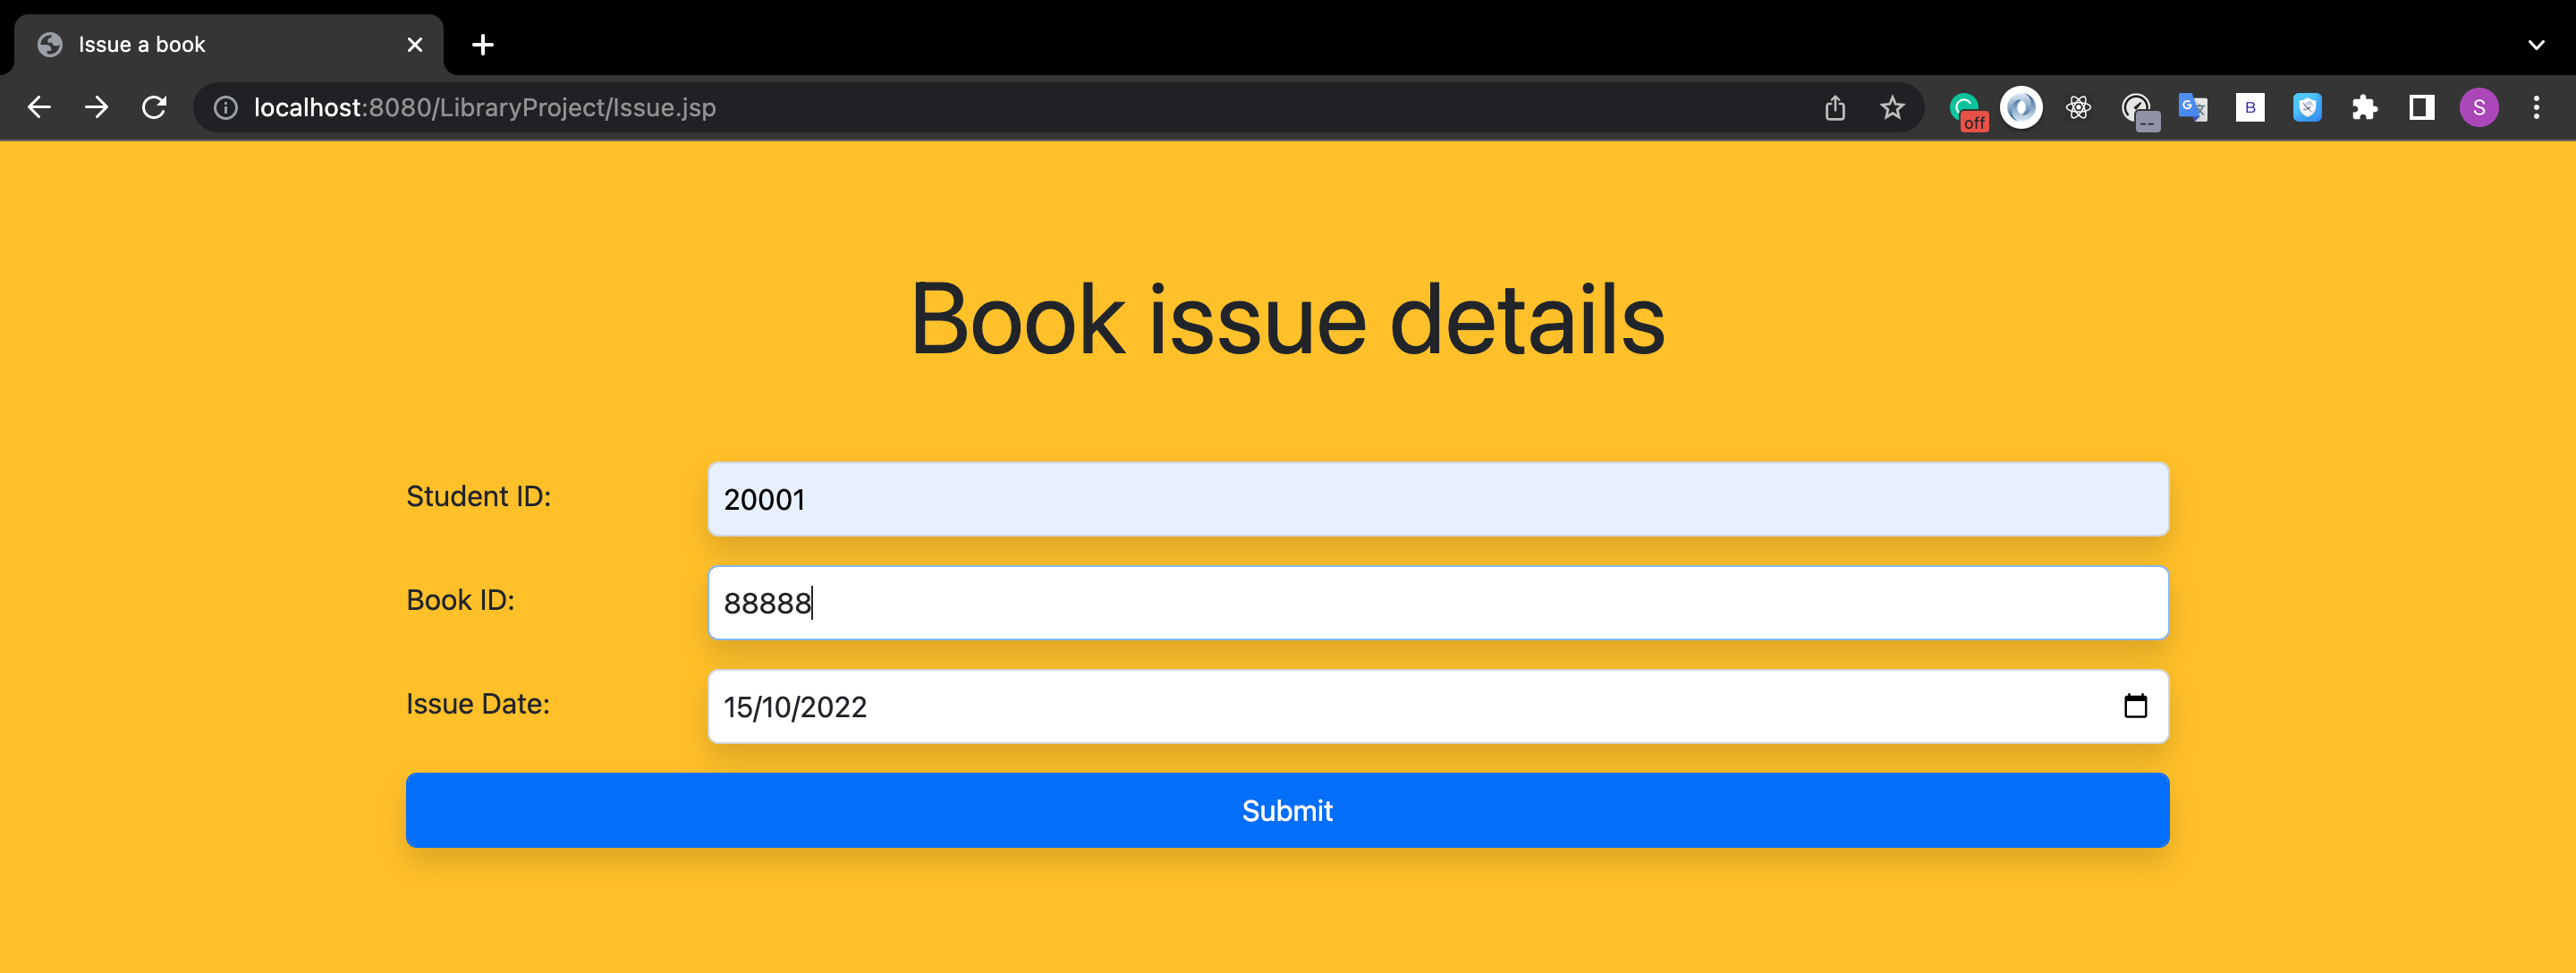
\includegraphics[scale=0.34]{screenshots/b3_16.png}
    \label{fig:my_label1}
    \caption{Issue.jsp with the inputs}
\end{figure}
\vspace{2cm}
\begin{figure}[!hbt]
    \centering
    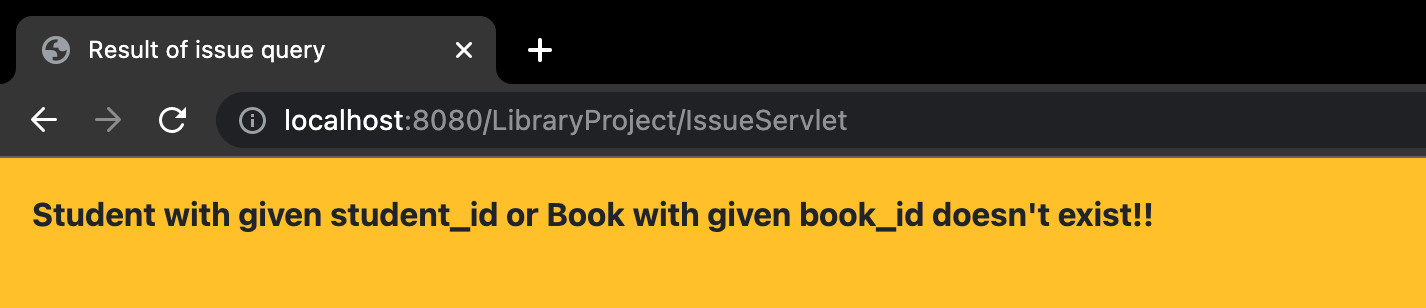
\includegraphics[scale=0.69]{screenshots/b3_17.png}
    \label{fig:my_label1}
    \caption{IssueResultException.jsp with result of issue query}
\end{figure}

\newpage


\end{document}